最初,C++通常认为是C语言的继承者,然而当前的C++已经演变成巨大的,有时可怕,甚至不可驯服的东西。随着语言的更新,则需要更多时间和耐心来了解它。我们将从基本结构开始,比如:数据类型、条件语句和循环语句、指针、结构和函数。并从底层系统程序员的角度来看这些结构,他们对计算机如何执行一条简单的指令感到好奇。深入理解这些基本结构是为更高级的抽象(如面向对象编程),以及为后续学习打下良好基础的必要条件。 \par
本章中,我们将了解以下内容: \par

\begin{itemize}
	\item 程序执行的细节及其入口点
	\item main()函数的特殊属性
	\item 函数调用和递归背后的复杂性
	\item 内存段和寻址基础
	\item 数据类型以及变量如何驻留在内存中
	\item 指针和数组
	\item 条件语句和循环的细节
\end{itemize}

\noindent\textbf{}\ \par
\textbf{编译器要求} \ \par
g++编译器需要添加编译选项 \texttt{-std=c++2a} 来编译本章的代码。可以从这里获取本章的源码文件:https:/​/github.​com/PacktPublishing/Expert-CPP \par

\noindent\textbf{}\ \par
\textbf{运行程序} \ \par
第1章中,我们了解了编译器在编译源代码后,如何生成一个可执行文件。可执行文件包含机器码,这些机器码可以复制到计算机内存中,由中央处理器(CPU)运行。复制是由操作系统内部的加载器完成。因此,操作系统(OS)将程序的内容复制到内存中,并通过向CPU传递条指令开始执行程序。 \par

\noindent\textbf{}\ \par
\textbf{main()} \ \par
程序的执行从main()函数开始,这是标准中规定的程序的指定入口。一个简单的程序输出\texttt{Hello, World!}消息是这样的: \par

\begin{lstlisting}[caption={}]
#include <iostream>
int main() {
	std::cout << "Hello, World!" << std::endl;
	return 0;
}	
\end{lstlisting}

程序中main()函数的参数有两个,argc和argv,允许从环境中传递字符串,通常称为命令行参数。 \par
argc和argv是常规名称,可以用任何你想要的名称替换。argc参数保存了传递给main()函数的命令行参数的数量,argv参数保存参数具体信息: \par

\begin{lstlisting}[caption={}]
#include <iostream>
int main(int argc, char* argv[]) {
	std::cout << "The number of passed arguments is: " << argc << std::endl;
	std::cout << "Arguments are: " << std::endl;
	for (int ix = 1; ix < argc; ++ix) {
		std::cout << argv[ix] << std::endl;
	}
	return 0;
}
\end{lstlisting}

例如,我们可以用以下参数运行前面的示例: \par

\texttt{\$ my-program argument1 hello world --some-option}

输出如下所示:

\begin{lstlisting}[caption={}]
	The number of passed arguments is: 5 
	Arguments are: 
	argument1 
	hello 
	world 
	--some-option 
\end{lstlisting}

查看参数的数量时,是5个。第一个参数是程序名,这就是为什么在例子中跳过它,从第1个循环开始。 \par

\hspace*{\fill} \\ %插入空行

\includegraphics[width=0.05\textwidth]{images/tip}
很少会看到得到标准化的第三个参数,最常见的名称是envp。envp的类型是一个char指针数组,它保存着系统的环境变量。 \par

\noindent\textbf{}\ \par
程序可以包含许多函数,但总是从main()函数开始执行,至少从程序员的角度来看是这样。我们尝试编译以下代码: \par

\begin{lstlisting}[caption={}]
#include <iostream>
void foo() {
	std::cout << "Risky foo" << std::endl;
}
// trying to call the foo() outside of the main() function
foo();
int main() {
	std::cout << "Calling main" << std::endl;
	return 0;
}
\end{lstlisting}

g++在foo()上报出错误:\texttt{  C++ requires a type specifier for all declarations.}。调用解析为声明,而不是要执行的指令。对于经验丰富的开发人员来说,尝试在main()之前调用函数的方式看起来很愚蠢,所以让尝试另一种方式。如果声明了一个在初始化过程中调用函数呢?下面的例子中,定义了一个BeforeMain结构,构造函数打印一条消息,然后在全局作用域中声明BeforeMain类型的对象: \par

\begin{lstlisting}[caption={}]
#include <iostream>
struct BeforeMain {
	BeforeMain() {
		std::cout << "Constructing BeforeMain" << std::endl;
	}
};
BeforeMain b;
int main() {
	std::cout << "Calling main()" << std::endl;
	return 0;
}
\end{lstlisting}

示例成功编译,程序输出如下信息: \par

\begin{lstlisting}[caption={}]
Constructing BeforeMain
Calling main()
\end{lstlisting}

如果我们向BeforeMain添加一个成员函数并尝试调用它,会怎么样? \par

\begin{lstlisting}[caption={}]
struct BeforeMain {
	// constructor code omitted for brevity
	void test() {
		std::cout << "test function" << std::endl;
	}
};
BeforeMain b;
b.test(); // compiler error
int main() {
	// code omitted for brevity
}
\end{lstlisting}

test()的调用不会成功。不能在main()之前调用函数,但可以声明变量——有默认初始化的对象。实际程序中,会有一些东西需要在main()之前进行初始化。事实证明,main()函数并不是程序的真正起点。程序的实际启动函数准备环境,收集传递给程序的参数,然后调用main()函数。因为C++支持全局对象和静态对象,需要在程序开始之前(即main()函数被调用之前)进行初始化。在Linux世界中,这个函数被称为\underline{~~}libc\underline{ }start\underline{ }main。编译器使用\underline{~~}libc\underline{ }start\underline{ }main调用来生成的代码,该函数在main()函数调用之前可能(不)调用其他初始化函数。想象一下前面的代码将被修改成类似下面的样子: \par

\begin{lstlisting}[caption={}]
void __libc_start_main() {
	BeforeMain b;
	main();
}
__libc_start_main(); // call the entry point
\end{lstlisting}

我们将在接下来的章节中更详细地研究这个入口点。\par

\noindent\textbf{}\ \par
\textbf{main()的特质} \ \par
我们得出的结论是,main()实际上不是程序的入口点,尽管标准声明它是起点。编译器特别注意main()。它的行为就像一个常规的C++函数,但是除了作为第一个调用的函数之外,还有其他特殊的属性。首先,它是唯一可以省略return语句的函数: \par

\begin{lstlisting}[caption={}]
int main() {
	// works fine without a return statement
}
\end{lstlisting}

返回值表示执行状态。通过返回0,告诉控件main()已成功结束,因此如结束时没有遇到相应的return语句,则认为调用成功,效果与\texttt{return 0;}相同。 \par
main()函数的另一个有趣的特性是,它的返回类型不能自动推断。不允许使用auto类型说明符。下面是正则函数的工作原理: \par

\begin{lstlisting}[caption={}]
// C++11
auto foo() -> int {
	std::cout << "foo in alternative function syntax" << std::endl;
	return 0;
}

// C++14
auto foo() {
	std::cout << "In C++14 syntax" << std::endl;
	return 0;
}
\end{lstlisting}

通过auto,我们告诉编译器自动推断返回类型。在C++ 11中,我们还可以将类型名放在箭头后面(->),尽管第二种语法更短。考虑get\underline{ }ratio()函数,它是以整数形式返回: \par

\begin{lstlisting}[caption={}]
auto get_ratio(bool minimum) {
	if (minimum) {
		return 12; // deduces return type int
	}
	return 18; // fine: get_ratio's return type is already deduced to int
}
\end{lstlisting}

\hspace*{\fill} \\ %插入空行

\includegraphics[width=0.05\textwidth]{images/tip}
要成功地编译包含C++11、C++14、C++17或C++20新特性的C++代码,应该使用适当的编译器选项。使用g++进行编译时,使用\texttt{--std}标志并指定标准版本。推荐选项为\texttt{--std=c++2a}。 \par
\noindent\textbf{}\ \par

例子编译成功了,但是当我们对main()函数使用相同的方式时,看看会发生什么: \par

\begin{lstlisting}[caption={}]
auto main() {
	std::cout << get_ratio(true);
	return 0;
}
\end{lstlisting}

编译器将产生以下错误: \par

\begin{itemize}
	\item \texttt{cannot initialize return object of type 'auto' with an rvalue 	of type 'int'}
	\item \texttt{'main' must return 'int' .}
\end{itemize}

main()函数发生了一些奇怪的事情。这是因为main()函数允许省略return语句,但对于编译器来说,必须存在return语句才能支持自动返回类型推断。 \par
如果有多个return语句,必须推断成相同的类型。假设我们需要更新这个函数的版本,它返回一个整数值(如前面的例子所示)。如果指定了返回类型,则返回一个更精确的浮点值: \par

\begin{lstlisting}[caption={}]
auto get_ratio(bool precise = false) {
	if (precise) {
		// returns a float value
		return 4.114f;
	}
	return 4; // returns an int value
}
\end{lstlisting}

上面的代码不能成功编译的原因是,有两个具有不同推断类型的return语句。 \par

\noindent\textbf{}\ \par
\textbf{constexpr} \ \par
constexpr声明函数的值可以在编译时求值,也适用于变量。名称本身由const和表达式组成。这是一个有用的特性,允许最大限度地优化代码。来看看下面的例子: \par

\begin{lstlisting}[caption={}]
int double_it(int number) {
	return number * 2;
}
constexpr int triple_it(int number) {
	return number * 3;
}
int main() {
	int doubled = double_it(42);
	int tripled = triple_it(42);
	int test{0};
	std::cin >> test;
	int another_tripled = triple_it(test);
}
\end{lstlisting}

看看在前面的例子中,编译器是如何修改main()函数的。假设编译器不能优化double\underline{ }it()函数(内联函数),main()函数将采用以下形式: \par

\begin{lstlisting}[caption={}]
int main() {
	int doubled = double_it(42);
	int tripled = 126; // 42 * 3
	int test = 0;
	std::cin >> test;
	int another_tripled = triple_it(test);
}
\end{lstlisting}

constexpr不能保证在编译时计算函数值。如果在编译时知道constexpr函数的输入,编译器就可以这样做。这就是前面的直接转换为tripled变量的计算值126,并且对another\underline{ }tripled变量没有影响的原因。 \par

\hspace*{\fill} \\ %插入空行

\includegraphics[width=0.05\textwidth]{images/tip}
C++ 20引入了consteval说明符,允许在编译时对函数结果求值。换句话说,consteval函数在编译时产生一个常量表达式。说明符使函数成为即时函数,如果函数调用不能导致常量表达式,则会产生错误。注意:main()函数不能声明为constexpr。 \par
\noindent\textbf{}\ \par

C++20还引入了constinit说明符。我们使用constinit声明一个具有静态或线程存储持续时间的变量。我们将在第8章中讨论线程存储持续时间。与constinit的区别是,因为constexpr要求对象具有静态初始化和常量销毁,所以可以将它用于没有constexpr析构函数的对象。而且,constexpr使对象具有const限定条件,而constinit则没有。然而,constinit要求对象具有静态初始化的能力。 \par

\noindent\textbf{}\ \par
\textbf{递归} \ \par
main()的另一个特性是不能递归调用。从操作系统的角度来看,main()函数是程序的入口点,所以再次调用它将意味着一切重新开,因此是禁止的。例如,print\underline{ }number()函数进行递归调用的话,就无法停止了: \par

\begin{lstlisting}[caption={}]
void print_number(int num) {
	std::cout << num << std::endl;
	print_number(num + 1); // recursive call
}
\end{lstlisting}

调用print\underline{ }number(1)函数将输出数字1、2、3等。这更像是一个无限调用自己的函数,而不是一个正确的递归函数。应该添加更多的属性,使print\underline{ }number()函数成为有用的递归函数。首先,递归函数必须有一个基本情况,即当进一步的函数调用stop时,这意味着停止递归。我们可以为print\underline{ }number()函数设置这样的情况,例如:打印100以下的所有数字: \par

\begin{lstlisting}[caption={}]
void print_number(int num) {
	if (num > 100) return; // base case
	std::cout << num << std::endl;
	print_number(num + 1); // recursive call
}
\end{lstlisting}

对于递归函数来说还有一个属性:使用基本方法将任务拆分成子任务解决。前面的例子中,我们已经解决了函数的一个任务,也就是打印一个数字。打印了一个数字之后,继续处理下一个任务:打印下一个数字,直到做完。函数调用自身并没有什么神奇之处,可以把它看作是一个函数,调用具有相同实现的另一个函数。真正有趣的是递归函数如何影响整个程序的执行:  \par

\begin{lstlisting}[caption={}]
int sum(int n, int m) { return n + m; }
int max(int x, int y) {
	int res = x > y ? x : y;
	return res;
}
int calculate(int a, int b) {
	return sum(a, b) + max(a, b);
}

int main() {
	auto result = calculate(11, 22);
	std::cout << result; // outputs 55
}
\end{lstlisting}

当调用一个函数时,分配内存空间给它的参数和局部变量。程序从main()函数开始,在本例中main()函数调用calculate()函数,并以11和12为参数。跳转到calculate()函数时,main()函数则处于暂停状态,并等待calculate()函数返回后继续执行。calculate()函数有两个参数a和b,尽管对sum()、max()和calculate()的形参进行了不同的命名,但可以在所有函数中使用相同的名称。我们假设一个int需要4个字节的内存,因此要成功执行calculate()函数至少需要8个字节。分配8个字节后,值11和22需要复制到相应的位置(详见下图):

\begin{center}
	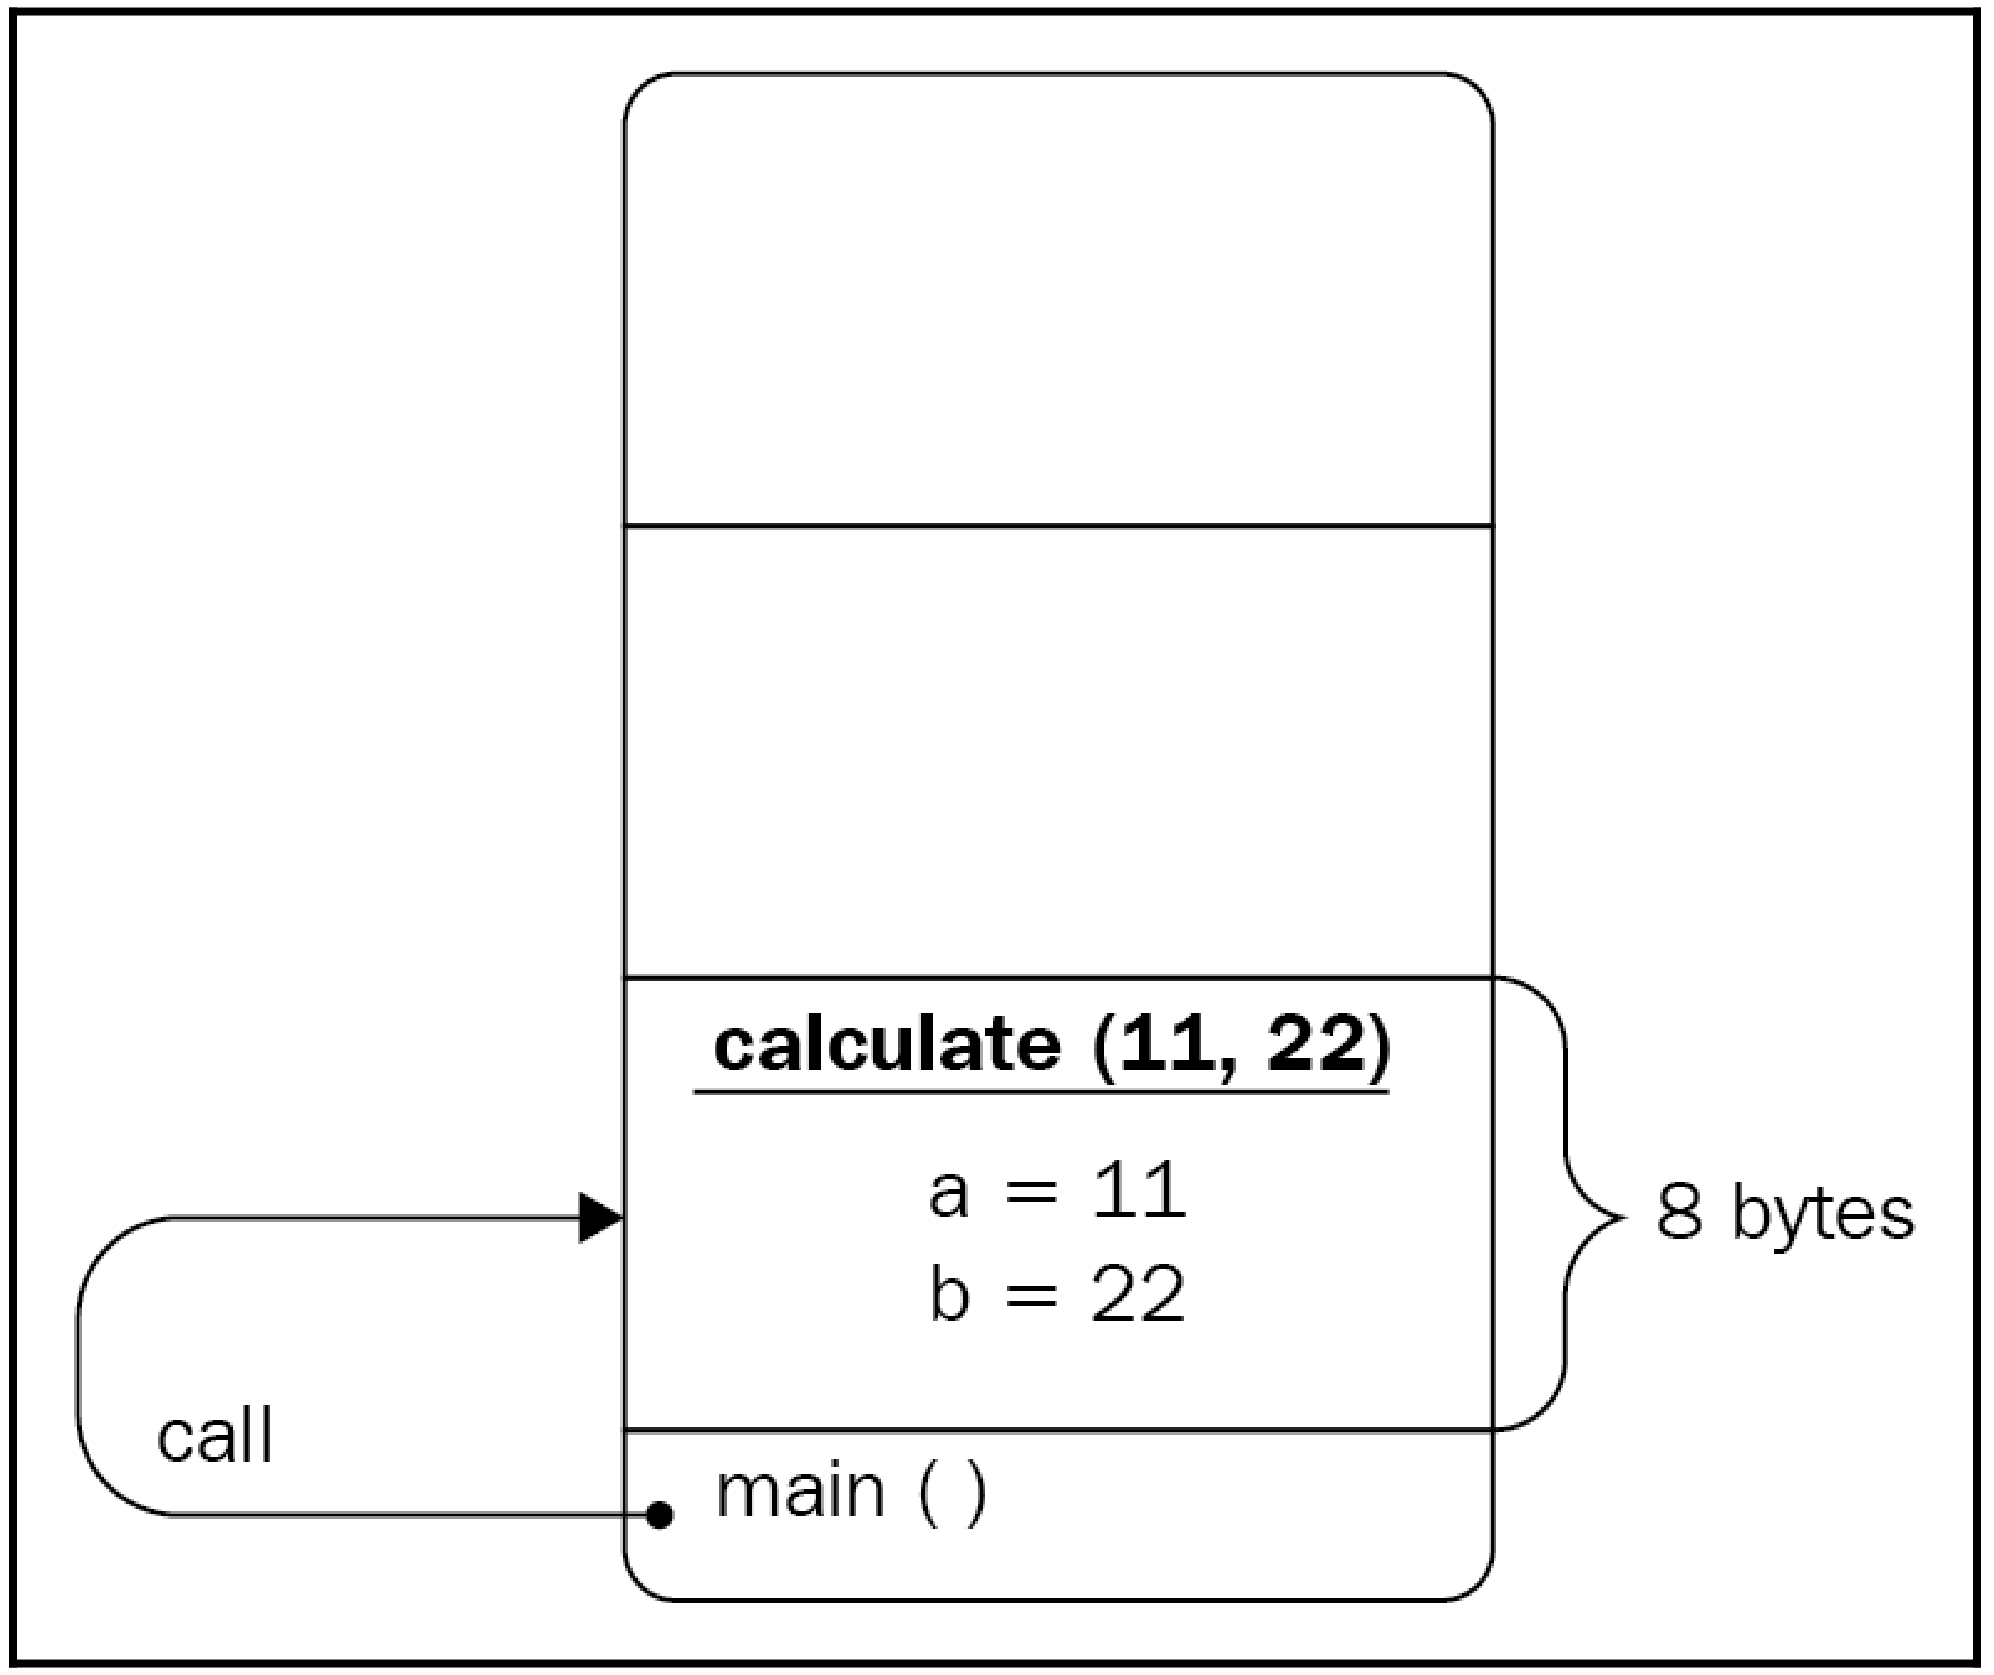
\includegraphics[width=0.4\textwidth]{content/Section-1/Chapter-2/1}
\end{center}

calculate()函数调用sum()和max(),并将参数值传递给它们。相应地,它会等待两个函数按顺序执行,以便形成返回到main()的值。sum()和max()函数不会同时调用。首先,调用sum(),这会导致将变量a和b的值复制到为sum()的参数(命名为n和m)分配的位置,这两个参数总共占用8个字节。参考下面的图,以便更好地理解这一点: \par

\begin{center}
	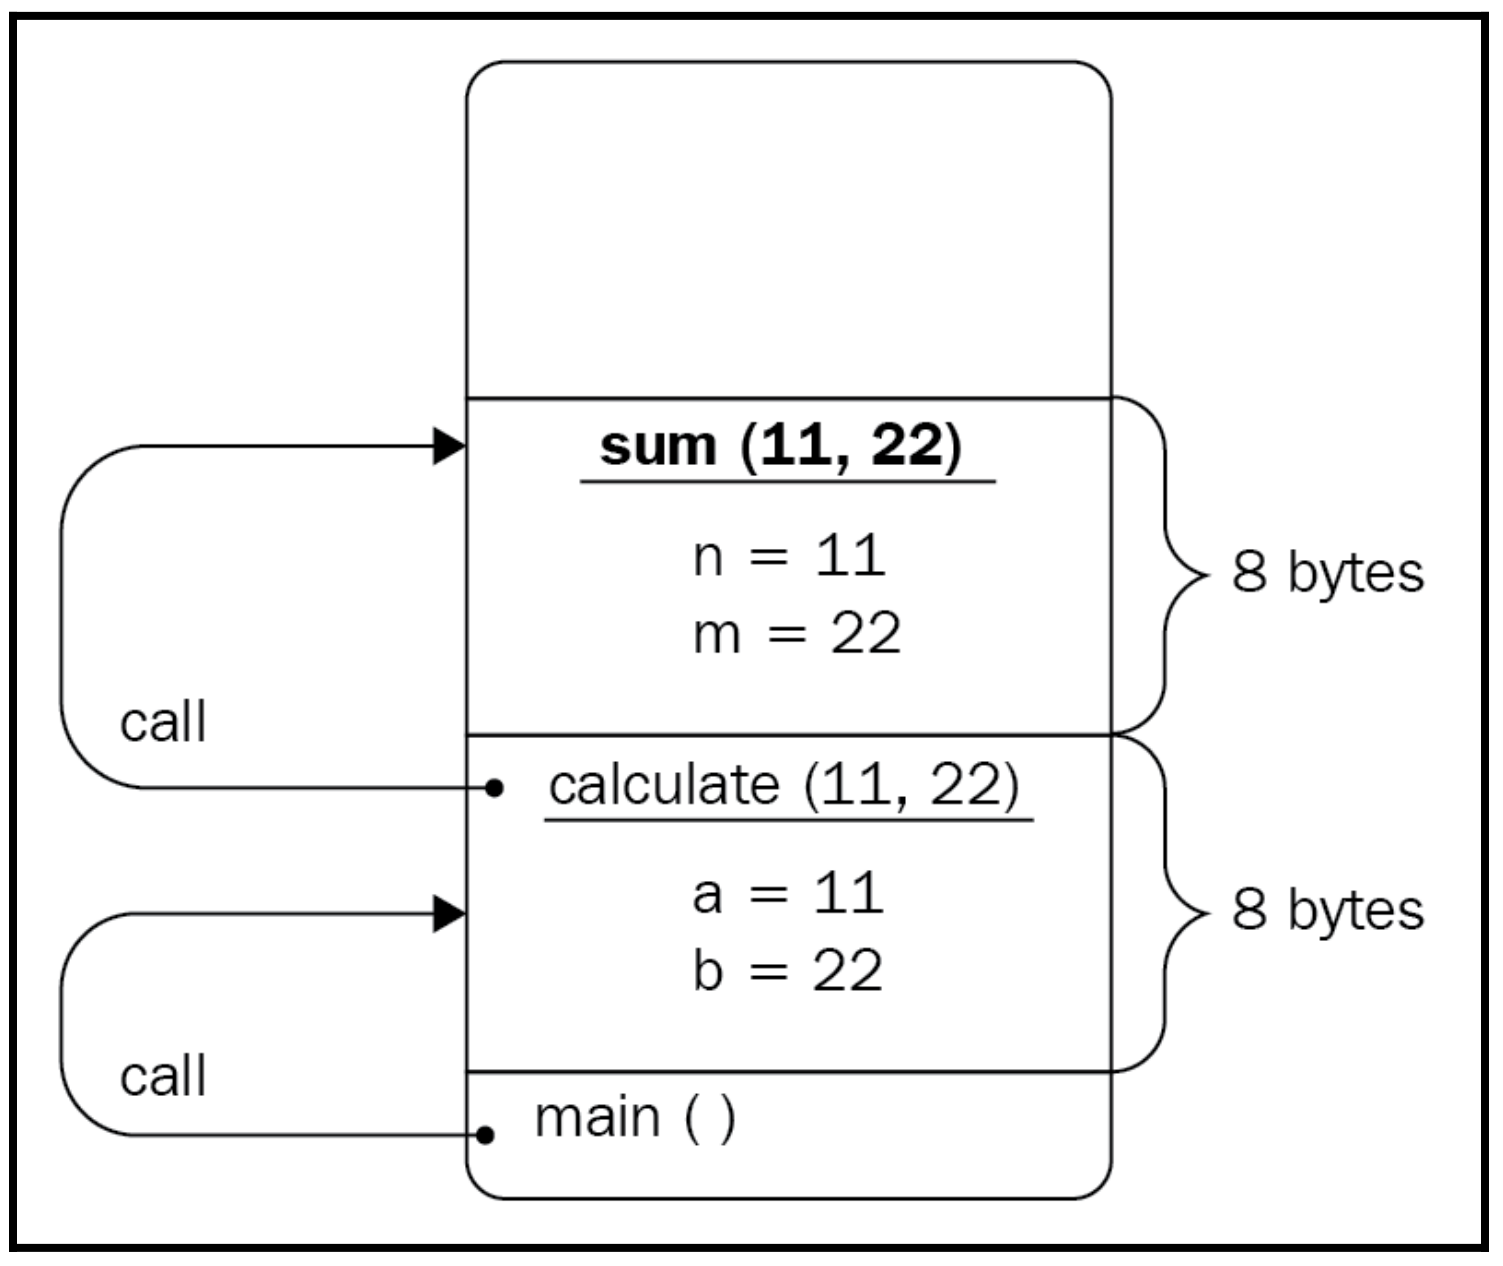
\includegraphics[width=0.4\textwidth]{content/Section-1/Chapter-2/2}
\end{center}

他们的总数经计算后返回。函数完成并返回一个值后,释放内存空间。这意味着变量n和m不再是可访问的,它们的空间可以重用。 \par

\hspace*{\fill} \\ %插入空行

\includegraphics[width=0.05\textwidth]{images/tip}
我们现在不考虑临时变量。稍后会重新讨论这个示例,以展示函数执行的细节,包括临时变量,以及如何尽可能地避免使用临时变量。 \par
\noindent\textbf{}\ \par

sum()返回一个值后,将调用max()函数。遵循相同的逻辑:内存分配给参数x和y,以及res变量。我们故意将三元操作符(?:)的结果存储在res中,以便让max()函数为本例分配更多空间。因此,总共为max()函数分配了12个字节。此时,main()函数仍处于等待状态,等待calculate()完成,而calculate()函数也处于等待状态,等待max()函数完成(详情见下图):\par

\begin{center}
	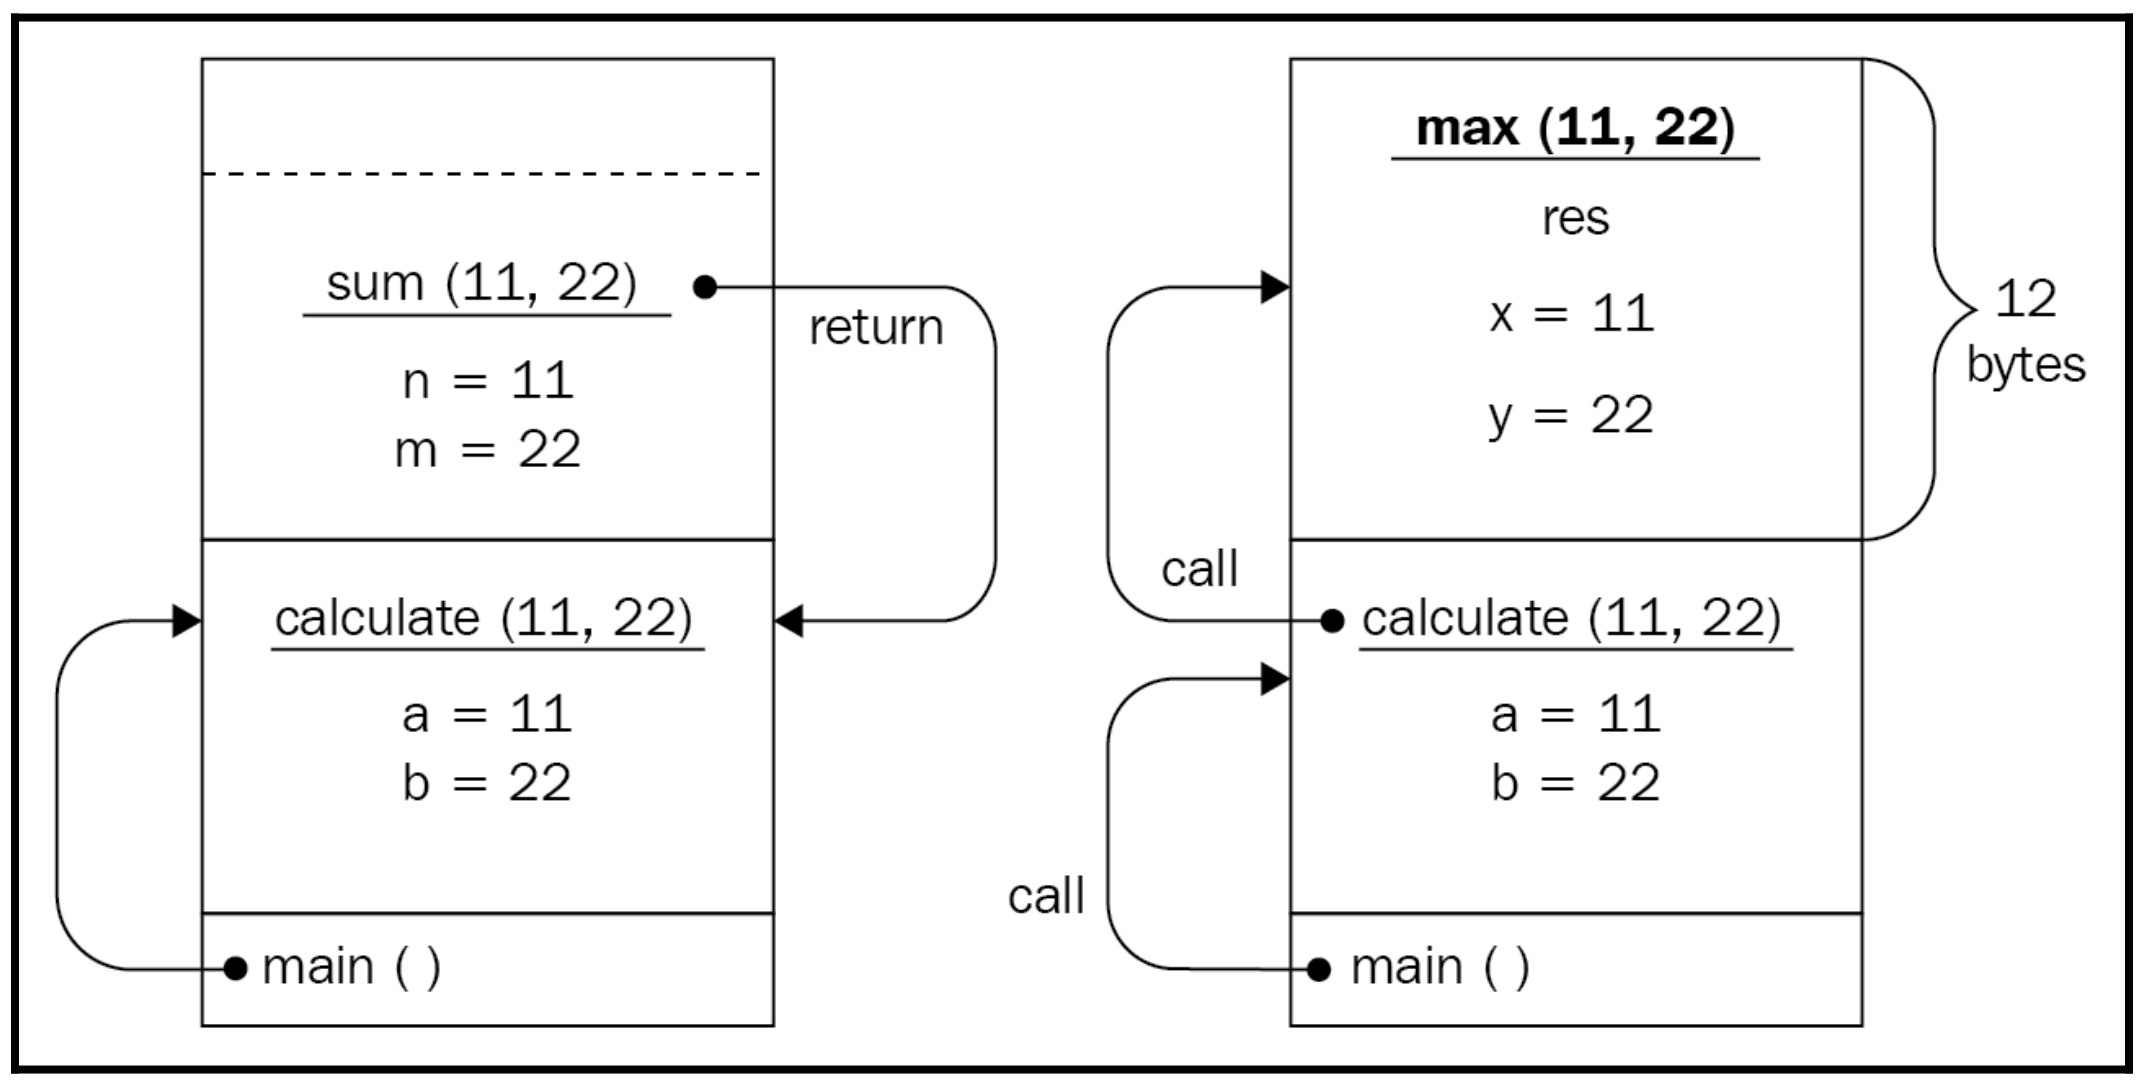
\includegraphics[width=0.5\textwidth]{content/Section-1/Chapter-2/3}
\end{center}

当max()完成时,分配给它的内存将被释放,并形成一个返回值。类似地,当calculate()返回时,内存被释放,main()函数的局部变量结果将包含calculate()返回的值\par
然后main()函数完成工作,程序退出,操作系统释放分配给该程序的内存,以后可在其他程序重用。为函数分配和释放内存(释放内存)的过程,是使用堆栈的概念来完成的。\par

\hspace*{\fill} \\ %插入空行

\includegraphics[width=0.05\textwidth]{images/tip}
堆栈是一个数据结构,它有自己插入和访问数据的规则。在函数调用的上下文中,堆栈通常用来提供给内存段,该程序根据堆栈数据结构的规则进行自我管理。我们将在本章后面更详细地讨论。 \par
\noindent\textbf{}\ \par

说回到递归,当函数调用自身时,应该为新调用的函数的参数和局部变量(如果有的话)分配内存。该函数再次调用自身,意味着堆栈将继续增长(为新函数提供空间)。我们调用相同的函数没有关系,从堆栈的角度来看,每个新的调用都是对一个完全不同的函数的调用,因此它一边哼着自己最喜欢的小调,一边分配空间。请看下面的图表: \par

\begin{center}
	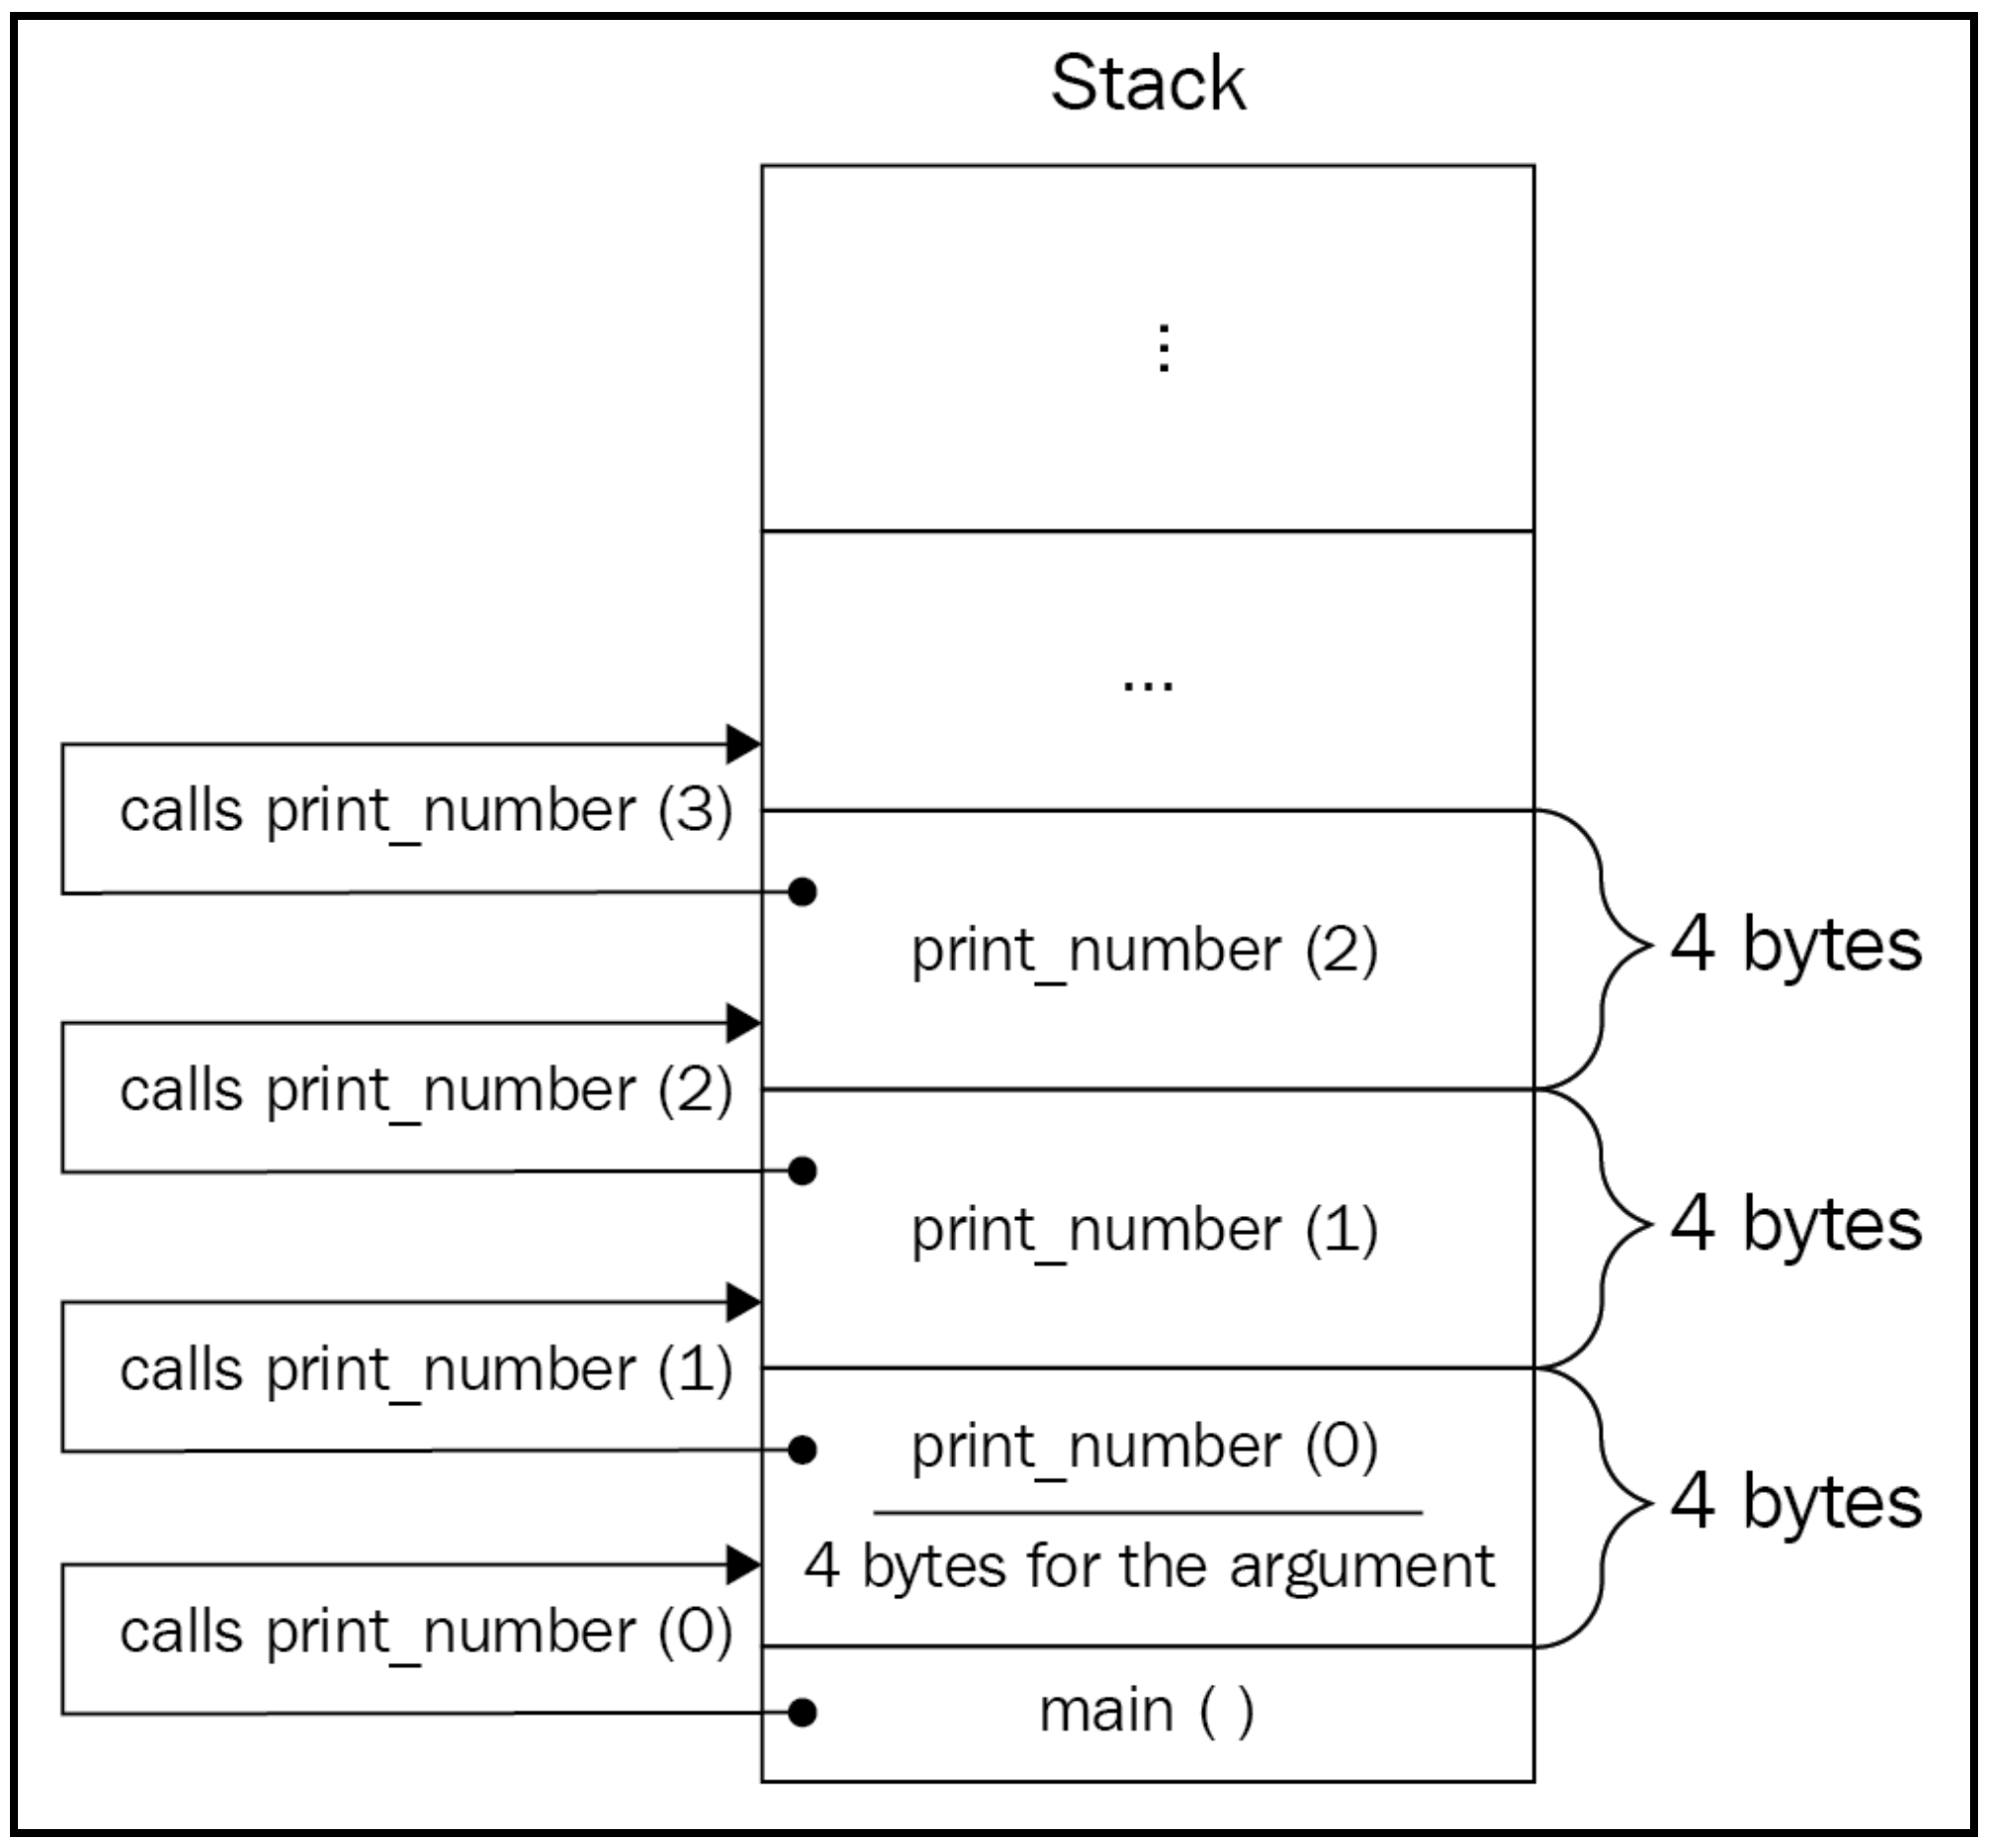
\includegraphics[width=0.5\textwidth]{content/Section-1/Chapter-2/4}
\end{center}

递归函数的第一次调用处于保持状态,并等待同一函数的第二次调用,后者又处于保持状态,并等待第三次调用完成并返回一个值,第三次调用又处于保持状态,依此类推。如果函数中有错误,或者递归基难以达到,堆栈会过度增长,将导致程序崩溃,这称为\textbf{堆栈溢出}。 \par

\hspace*{\fill} \\ %插入空行

\includegraphics[width=0.05\textwidth]{images/tip}
尽管递归为问题提供了优雅的解决方案,但请避免使用递归,并使用迭代方法(循环)进行替代。在关键任务系统开发指南,如火星探测器导航系统,完全禁止使用递归。\par
\noindent\textbf{}\ \par

第1章中,我们提到了协程。尽管在本书后面会有详细讨论,但需要注意的是主函数不能是协程。\par

\noindent\textbf{}\ \par
\textbf{处理数据} \ \par
当我们提到计算机内存时,我们会默认地想到随机存取存储器(RAM),而且RAM是SRAM或DRAM的通用术语,我们默认RAM是指DRAM,除非另有说明。为了清除这些东西,让我们看看下面的图表,它说明了内存的层次结构: \par

\begin{center}
	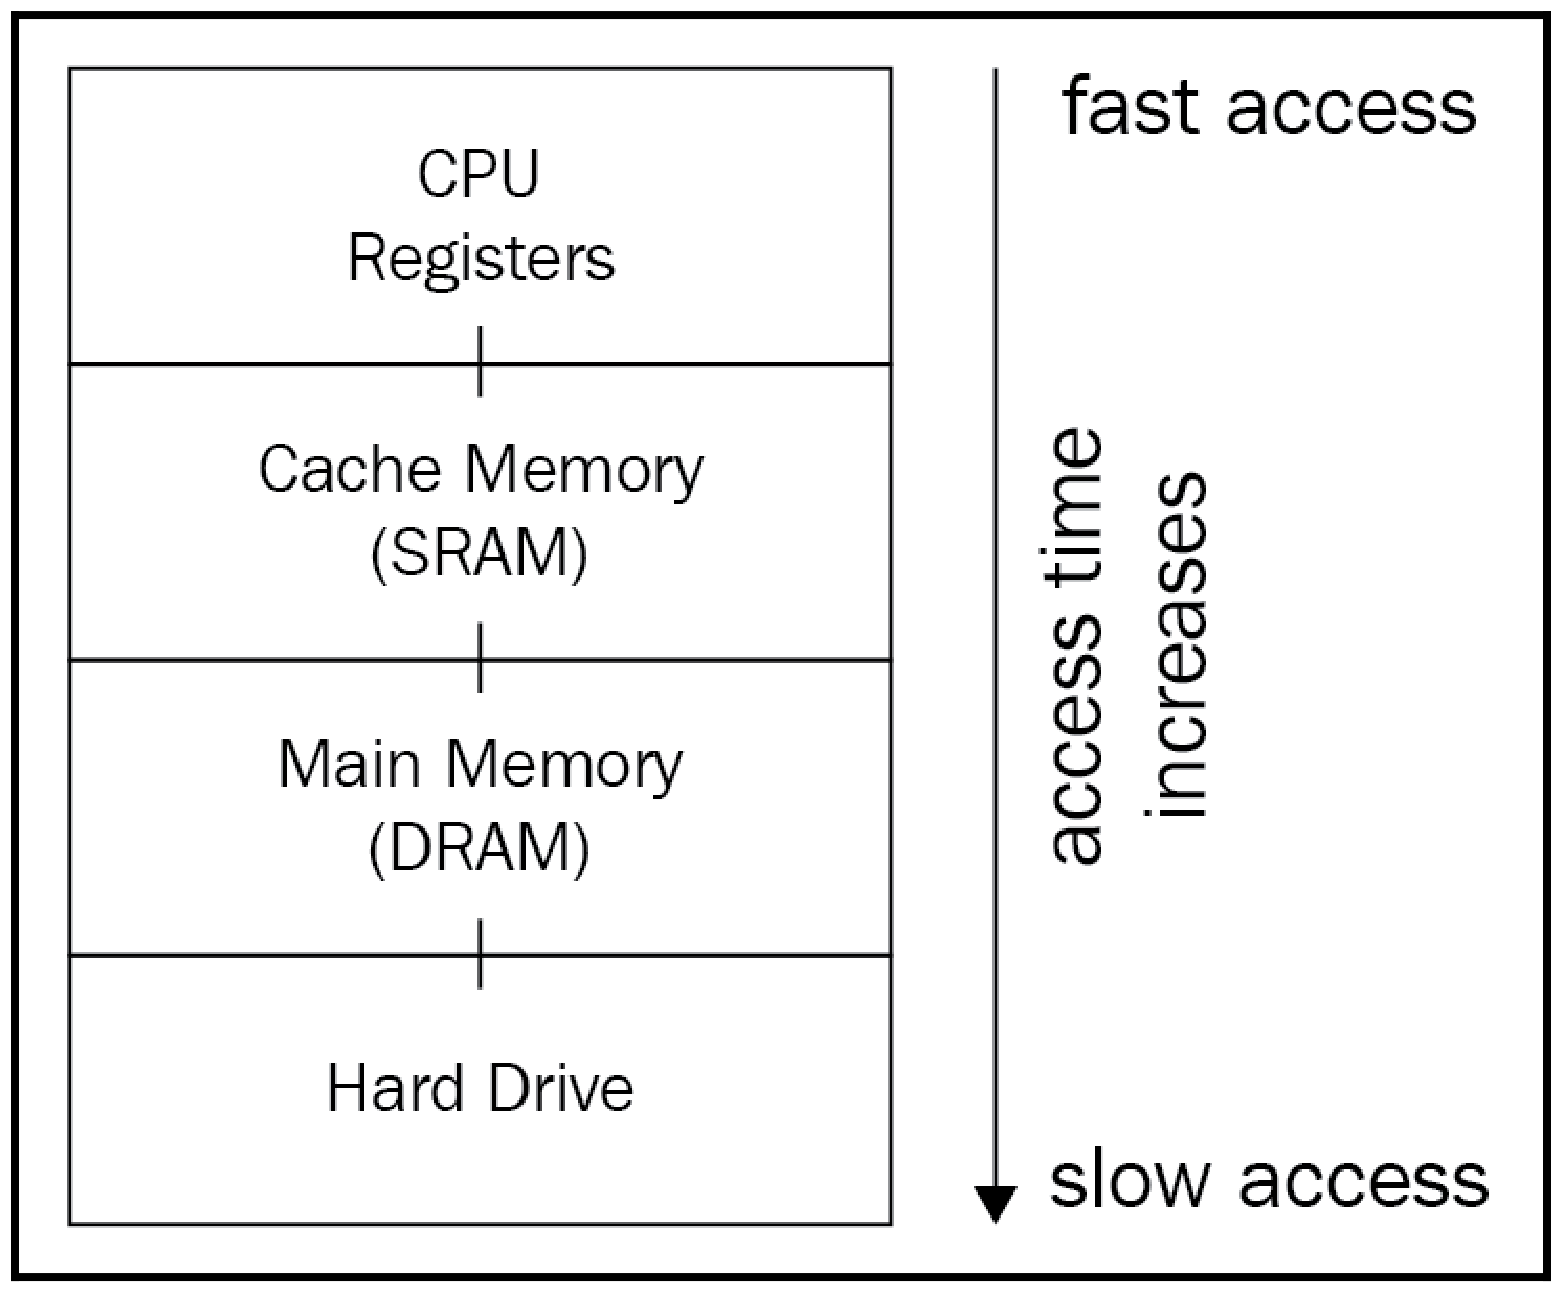
\includegraphics[width=0.5\textwidth]{content/Section-1/Chapter-2/5}
\end{center}

编译一个程序时,编译器将最终的可执行文件存储在硬盘驱动器中。为了运行可执行文件,指令加载到RAM中,然后由CPU一个个地执行。这使我们得出结论,任何需要执行的指令都应该在RAM中。其中,负责运行和监视程序的环境起着主要作用。 \par
我们编写的程序在宿主环境中执行,也就是在操作系统中。OS不直接将程序的内容(指令和数据,也就是进程)加载到RAM中,而是加载到虚拟内存中,这是一种可以方便处理进程和在进程之间共享资源的机制。当我们提到一个进程加载到的内存时,我们指的内存是虚拟内存,它会将进程的内容映射到RAM中。 \par

\hspace*{\fill} \\ %插入空行

\includegraphics[width=0.05\textwidth]{images/tip}
大多数时候,我们使用术语RAM、DRAM、虚拟内存和内存,认为虚拟内存是物理内存(DRAM)的一种抽象。\par
\noindent\textbf{}\ \par

首先介绍内存结构,然后了解内存中的数据类型。 \par

\noindent\textbf{}\ \par
\textbf{虚拟内存} \ \par
内存由许多盒子组成,每个盒子都能存储指定数量的数据。考虑到每个单元可以存储代表8位的1个字节,我们将把这些盒子称为内存单元。每个内存单元都是唯一的,即使它们存储相同的值。这种唯一性是通过对单元寻址来实现的,这样每个单元在内存中都有其唯一的地址。第一个单元格地址为0,第二个单元格地址为1,以此类推。\par
下面的图表是内存的一个摘录,每个单元都有其唯一的地址和存储1字节数据的能力:\par

\begin{center}
	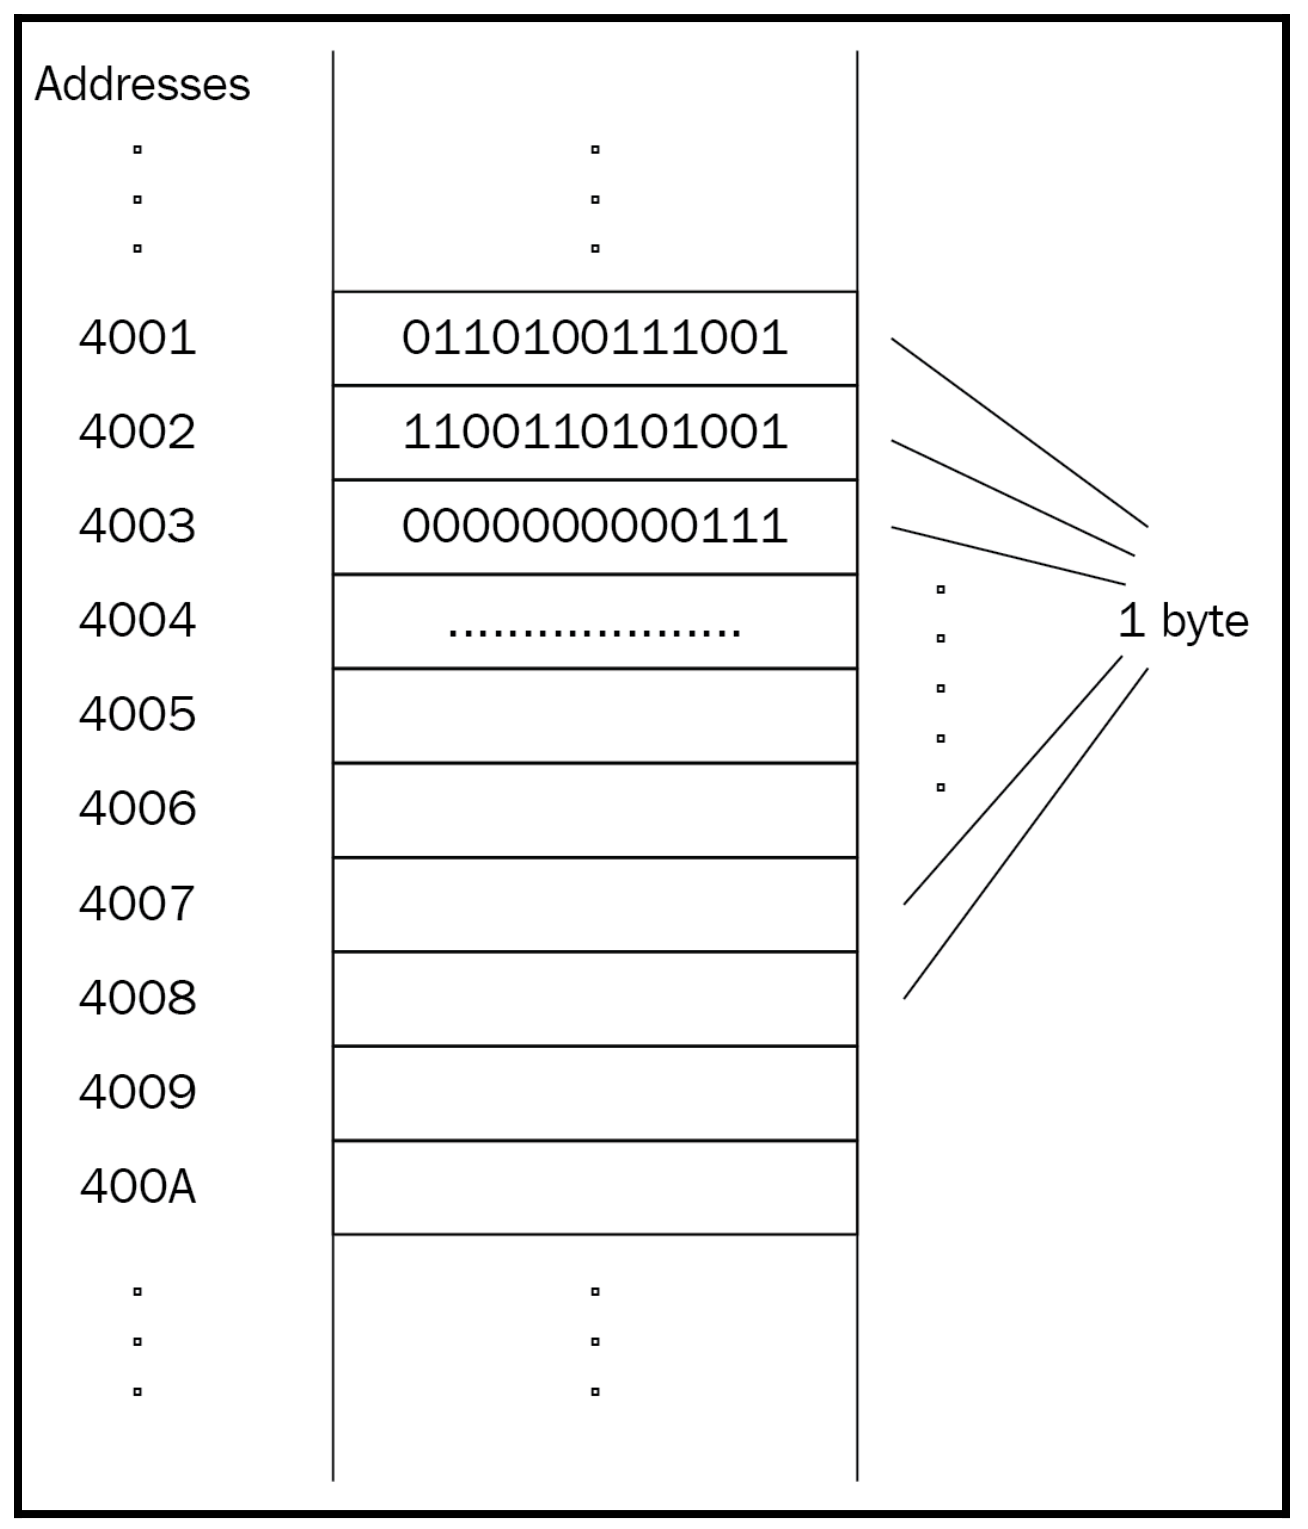
\includegraphics[width=0.5\textwidth]{content/Section-1/Chapter-2/6}
\end{center}

上图可以用来抽象地表示物理内存和虚拟内存。增加抽象层的目的是便于管理进程,并提供比物理内存更多的功能。例如,操作系统可以执行比物理内存大的程序。以一款电脑游戏为例,它的程序占用了将近2 GB的空间,而计算机的物理内存为512MB。虚拟内存允许操作系统通过从物理内存中卸载旧的部分,并映射新部分来部分地加载程序。 \par
虚拟内存还更好地支持内存中有多个程序,从而支持多个程序的并行(或伪并行)执行。这也提供了共享源码和数据的有效性,比如:动态库。当两个不同的程序需要使用相同的库时,这个库的单一实例可能存在于内存中,并在两个程序不知道对方的情况下使用。看看下面的图表,描述了加载到内存中的三个程序: \par

\begin{center}
	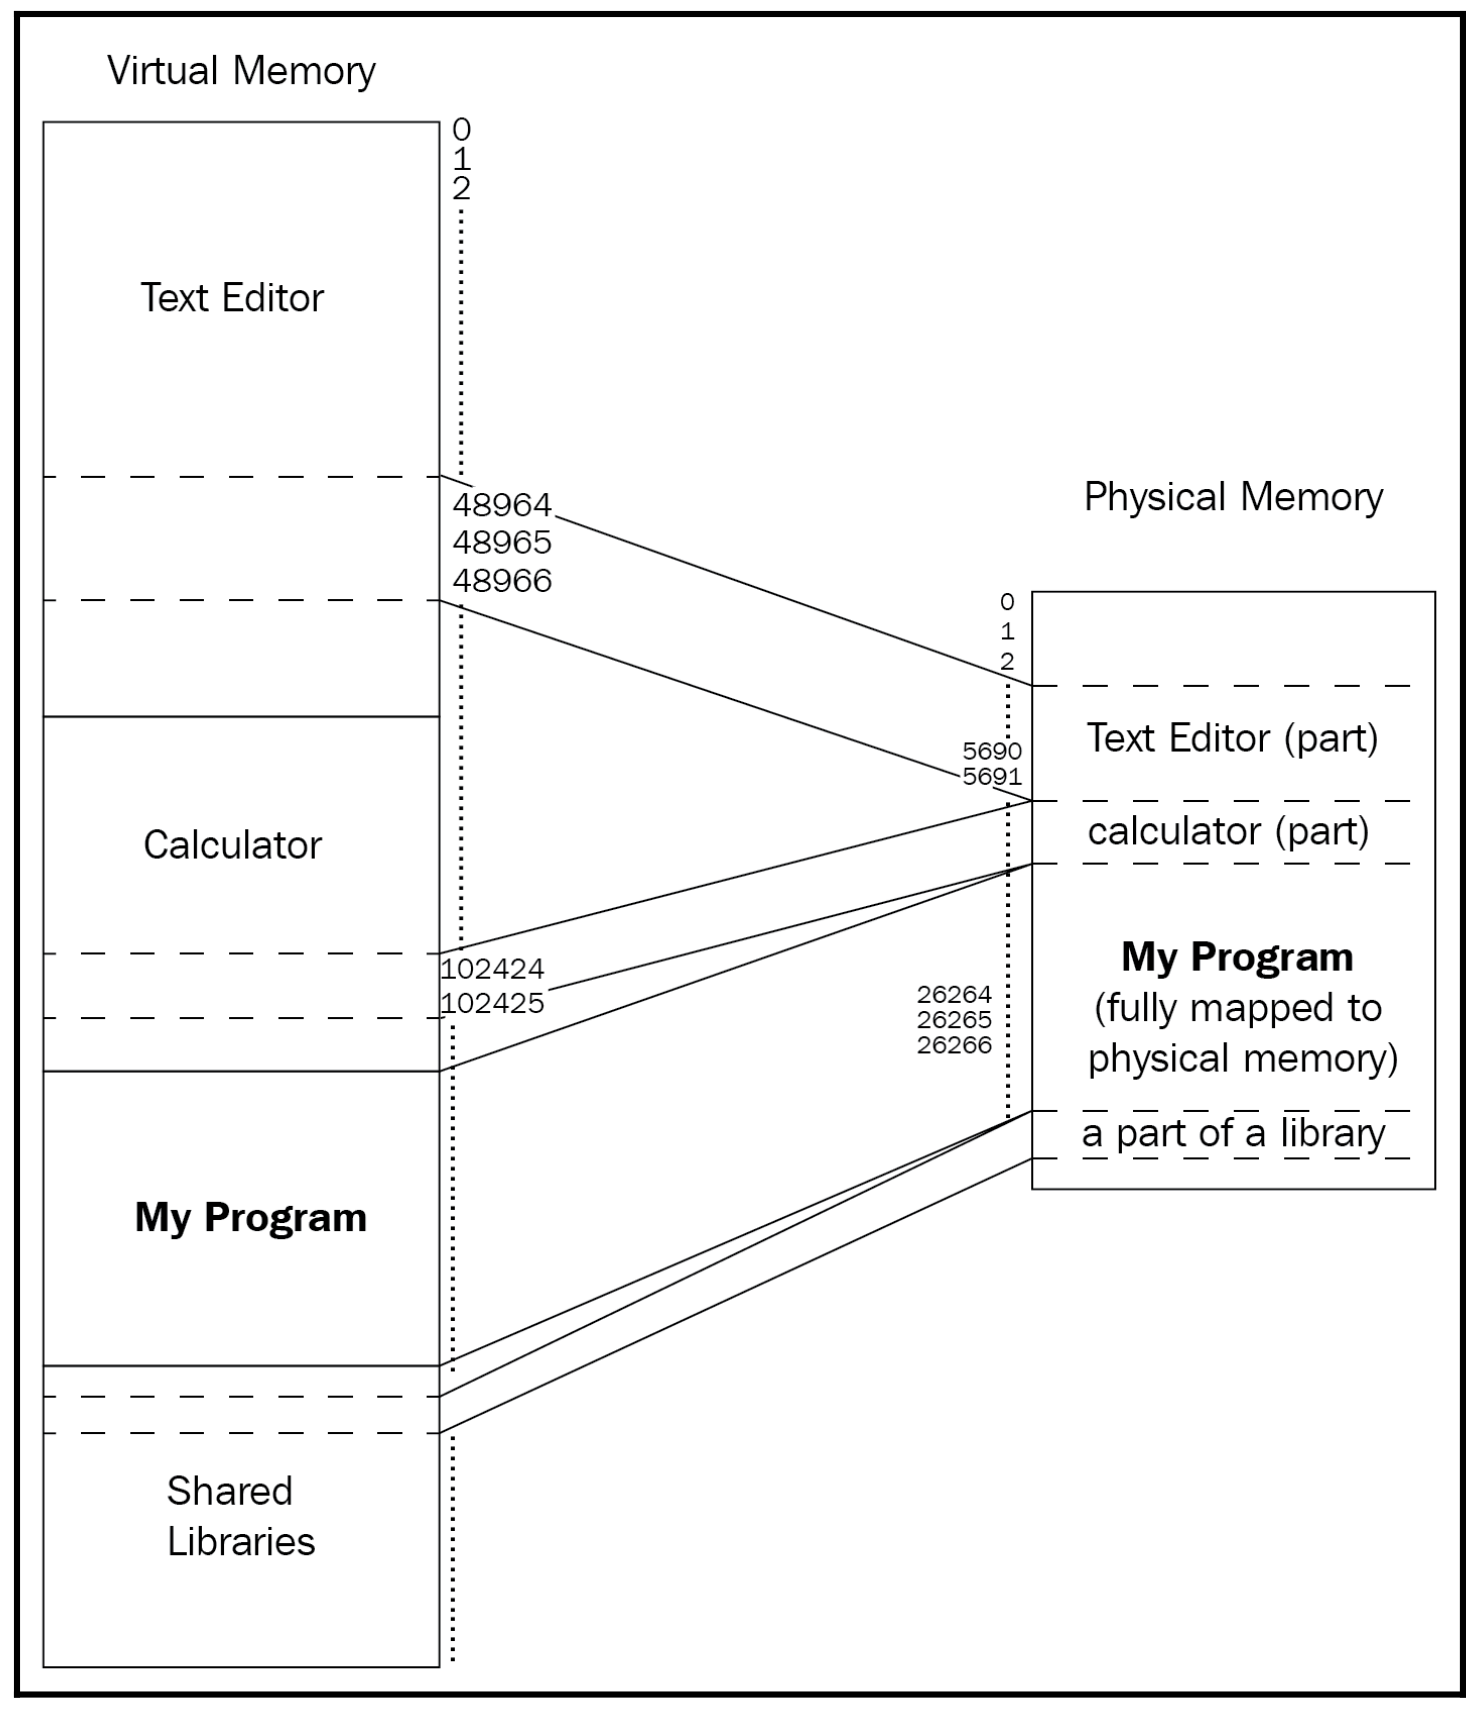
\includegraphics[width=0.8\textwidth]{content/Section-1/Chapter-2/7}
\end{center}

上图中有三个正在运行的程序,每个程序都占用虚拟内存中的一些空间。\textbf{My Program}完全包含在物理内存中,而\textbf{Calculator}和\textbf{Text Editor}只有部分进行了映射。 \par

\noindent\textbf{}\ \par
\textbf{地址} \ \par
如前所述,每个存储单元都有唯一地址,这是每个存储单元唯一性的保证。地址通常用十六进制表示,因为短,转换成二进制比转换成十进制更快。加载到虚拟内存中的程序操作并查看逻辑地址,这些地址也称为虚拟地址,由操作系统提供,在需要时将其转换为物理地址。为了优化转换,CPU提供了转换备用缓冲区,是内存管理单元(MMU)的一部分,转译后备缓冲器缓存虚拟地址到最新的物理地址。因此,有效的地址转换是一个软/硬件任务。我们将在第5章中深入研究地址结构和转换的细节。 \par
地址的长度定义了系统可以操作的内存的大小。当遇到与系统位数相关的语句时,它实际上是指地址的长度,即地址长度为32位或64位。地址越长,内存越大。为了把事情弄清楚,比较一下8位长的地址和32位长的地址。正如前面约定,每个内存单元能够存储1个字节的数据,并且有唯一的地址。如果地址长度为8位,则第一个存储单元的地址全部为0 —— 0000 0000。下一个单元的地址要大1,也就是说,它是0000 0001,以此类推。 \par
可以用8位表示的最大值是1111 1111。那么,有多少内存单元可以用8位的地址长度表示呢?这个问题值得更详细地回答。1位可以表示多少个不同的值?两个!为什么如此?因为1位既可以表示1也可以表示0。2位可以表示多少不同的值?00是一个值,01是另一个值,10,最后是11。所以,总共四个不同的值可以用2位表示。让我们做一个表格: \par

\begin{center}
	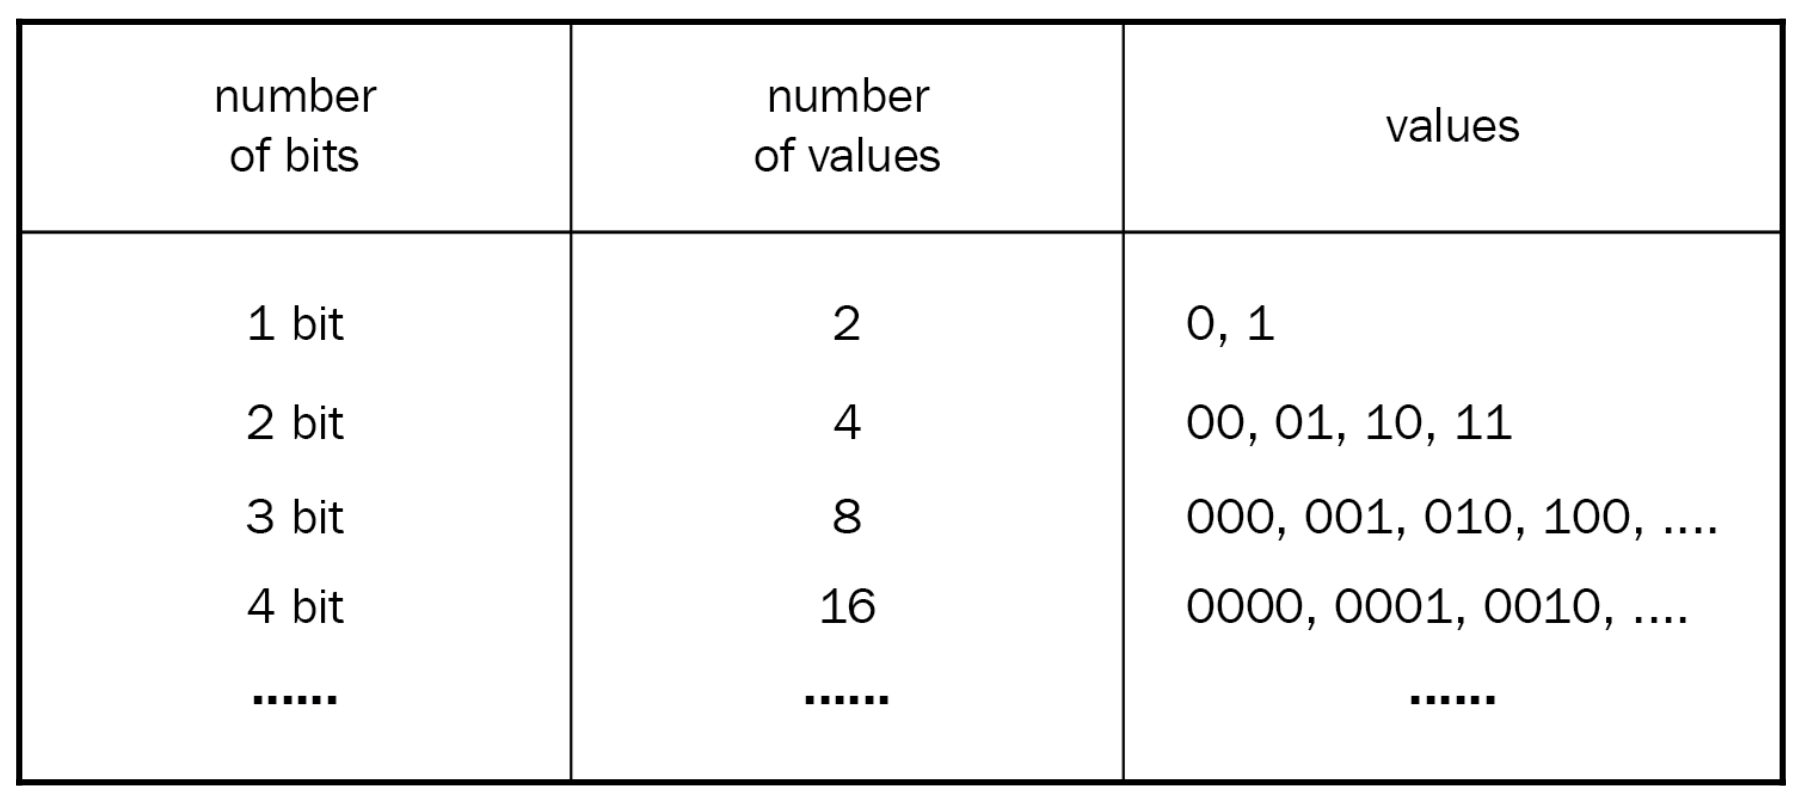
\includegraphics[width=0.5\textwidth]{content/Section-1/Chapter-2/8}
\end{center}

我们可以在这里看到一个模式。一个数字的每个位置(每个比特)可以表示两个值,因此可以通过求$2^N$来计算N位所代表的不同值的数量。因此,用8位表示的不同值的个数是$2^8 = 256$。这意味着一个8位系统可以寻址256个内存单元。另一方面,32位系统能够寻址$2^{32} = 4294967296$个内存单元,每个单元存储1字节的数据,即存储$4294967296 * 1byte= 4GB$的数据。

\noindent\textbf{}\ \par
\textbf{数据类型} \ \par
数据类型有什么意义呢?为什么我们不能在C++中使用一些var关键字来声明变量,而忘记诸如short, long, int, char, wchar等变量呢?C++也支持类似的结构,本章之前已经使用过的auto关键字,也就是所谓的占位符类型说明符。我们不能(也绝不能)声明一个变量,然后在运行时改变它的类型。下面的代码可能是有效的JavaScript代码,但绝对不是有效的C++代码: \par

\begin{lstlisting}[caption={}]
var a = 12;
a = "Hello, World!";
a = 3.14;
\end{lstlisting}

假设C++编译器可以编译这段代码。应该为变量a分配多少字节的内存?当声明\texttt{var a = 12;}时,编译器可以将其类型推断为int,并指定4个字节的内存空间,但当变量将其值更改为\texttt{Hello, World!},编译器必须重新分配空间,或者创建一个新的名为a1的std::string类型的隐藏变量。然后,编译器尝试查找代码中,以字符串而不是整数或double形式访问变量的每个访问,并用隐藏的a1变量。编译器可能会退出并开始思考生命周期的意义。 \par
我们可以在C++中声明类似于前面的代码,如下所示: \par

\begin{lstlisting}[caption={}]
auto a = 12;
auto b = "Hello, World!";
auto c = 3.14;
\end{lstlisting}

前两个示例的区别在于,第二个示例声明了三种不同类型的三个不同变量。前面的非C++代码只声明了一个变量,然后将不同类型的值赋给它。在C++中,不能更改变量的类型,但是编译器允许使用自动占位符,并根据赋给该变量的值推断变量的类型。\par
理解类型是在编译时推导出来的至关重要,而像JavaScript这样的语言则允许在运行时推导类型。后者是可能的,因为这类程序运行在虚拟机等环境中,而运行C++程序的环境是操作系统。C++编译器必须生成一个有效的可执行文件,该文件可以复制到内存中,并在没有支持系统的情况下运行。这迫使编译器预先知道变量的实际大小。知道大小对于生成最终的机器码很重要,因为访问变量需要地址和大小,给变量分配内存空间需要它应占用的字节数。 \par
C++类型系统将类型分为两大类: \par

\begin{itemize}
	\item 基本类型(int, double, char, void)
	\item 复合类型(指针、数组、类)
\end{itemize}

C++甚至支持特殊的类型特征,可以使用std::is\underline{ }fundamental和std::is\underline{ }compound,确定类型的类别,例如:\par

\begin{lstlisting}[caption={}]
#include <iostream>
#include <type_traits>
struct Point {
	float x;
	float y;
};
int main() {
	std::cout << std::is_fundamental_v<Point> << " "
	<< std::is_fundamental_v<int> << " "
	<< std::is_compound_v<Point> << " "
	<< std::is_compound_v<int> << std::endl;
}
\end{lstlisting}

我们使用了std::is\underline{ }fundamental\underline{ }v和std::is\underline{ }compound\underline{ }v定义模板变量,定义如下: \par

\begin{lstlisting}[caption={}]
template <class T>
inline constexpr bool is_fundamental_v = is_fundamental<T>::value;
template <class T>
inline constexpr bool is_compound_v = is_compound<T>::value;
\end{lstlisting}

程序输出:0 1 1 0。\par

\hspace*{\fill} \\ %插入空行

\includegraphics[width=0.05\textwidth]{images/tip}
打印类型类别之前,可以使用std::boolalpha I/O操纵符来打印true或false,而不是1或0。 \par
\noindent\textbf{}\ \par

大多数基本类型是算术类型,如int或double,甚至char类型也是算术类型。它实际上保存的是一个数字而不是一个字符,例如:\par

\begin{lstlisting}[caption={}]
char ch = 65;
std::cout << ch; // prints A
\end{lstlisting}

一个char变量保存1个字节的数据,这意味着它可以表示256个不同的值(因为1个字节是8位,8位可以用$2^8$种方式表示一个数字)。如果使用1位作为符号位,例如:允许类型也支持负数,会怎么样?这样我们就剩下7位来表示实际值,同理,它允许表示$2^7$个不同的值,128个(包括0)不同的正数和相同数量的负数。如果不包含0,则有符号char的范围为-127到+127。这种有符号与无符号的表示形式适用于几乎所有的整型。 \par
例如,遇到一个int的大小是4个字节,这是32位,无符号可表示的数字范围为0到$2^{32}$在,有符号克表示的数字范围为$-2^{31}$到$+2^{31}$。 \par

\noindent\textbf{}\ \par
\textbf{指针} \ \par
C++是一种独特的语言,它提供了对底层细节(如变量地址)的访问。我们可以使用\&操作符获取程序中声明的任何变量的地址,如下所示:\par

\begin{lstlisting}[caption={}]
int answer = 42;
std::cout << &answer;
\end{lstlisting}

这段代码将输出类似这样的内容: \par

	\textbf{0x7ffee1bd2adc} \par
	
注意地址的十六进制表示。虽然这个值是一个整数,但它用来存储指针变量。指针只是一个能够存储地址值并支持*操作符(解引用)的变量,允许我们找到存储在地址上的实际值。 \par
例如,在前面的例子中,为了存储变量answer的地址,我们可以声明一个指针并给它分配地址: \par

\begin{lstlisting}[caption={}]
int* ptr = &answer;
\end{lstlisting}

变量answer声明为int,通常占用4个字节的内存空间,每个字节都有自己的唯一地址。我们可以得出answer变量有四个唯一的地址吗?嗯,有也不是。它确实获得四个不同但相邻的内存字节,但是当对变量使用address操作符时,它返回第一个字节的地址。让我们看一看声明了几个变量的部分代码,然后说明它们是如何放置在内存中的: \par

\begin{lstlisting}[caption={}]
int ivar = 26;
char ch = 't';
double d = 3.14;
\end{lstlisting}

数据类型的大小是由实现定义的,尽管C++标准规定了每种类型支持的最小值范围。假设实现为int提供了4个字节,为double提供了8个字节,为char提供了1个字节。前面代码的内存布局应该是这样的:\par

\begin{center}
	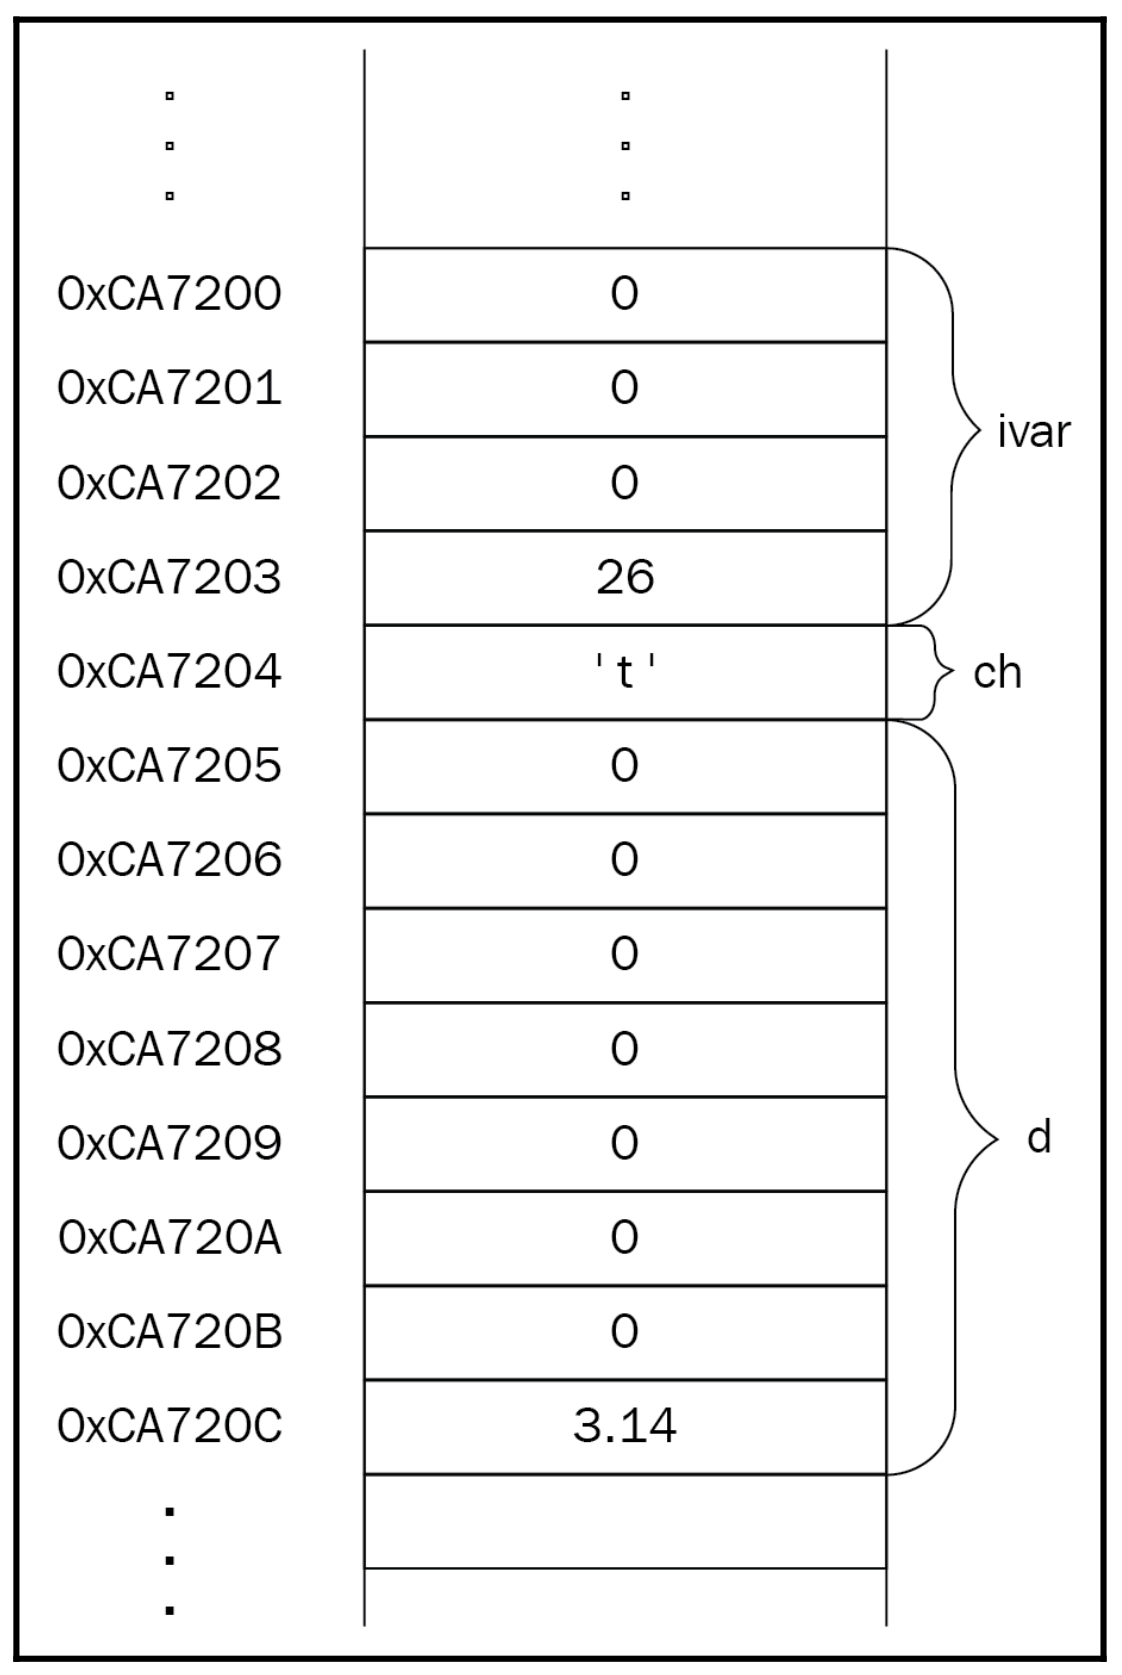
\includegraphics[width=0.5\textwidth]{content/Section-1/Chapter-2/9}
\end{center}

注意内存布局中的ivar,它存储在四个连续的字节中。 \par

当我们获取一个变量的地址时,无论它存储在单个字节还是多个字节中,我们都获得变量的第一个字节的地址。如果大小不影响寻址操作符背后的逻辑,那么为什么还要声明指针的类型呢?是为了在前面的例子中存储ivar的地址,所以将指针声明为int*:\par

\begin{lstlisting}[caption={}]
int* ptr = &ivar;
char* pch = &ch;
double* pd = &d;
\end{lstlisting}

上述代码如下图所示: \par

\begin{center}
	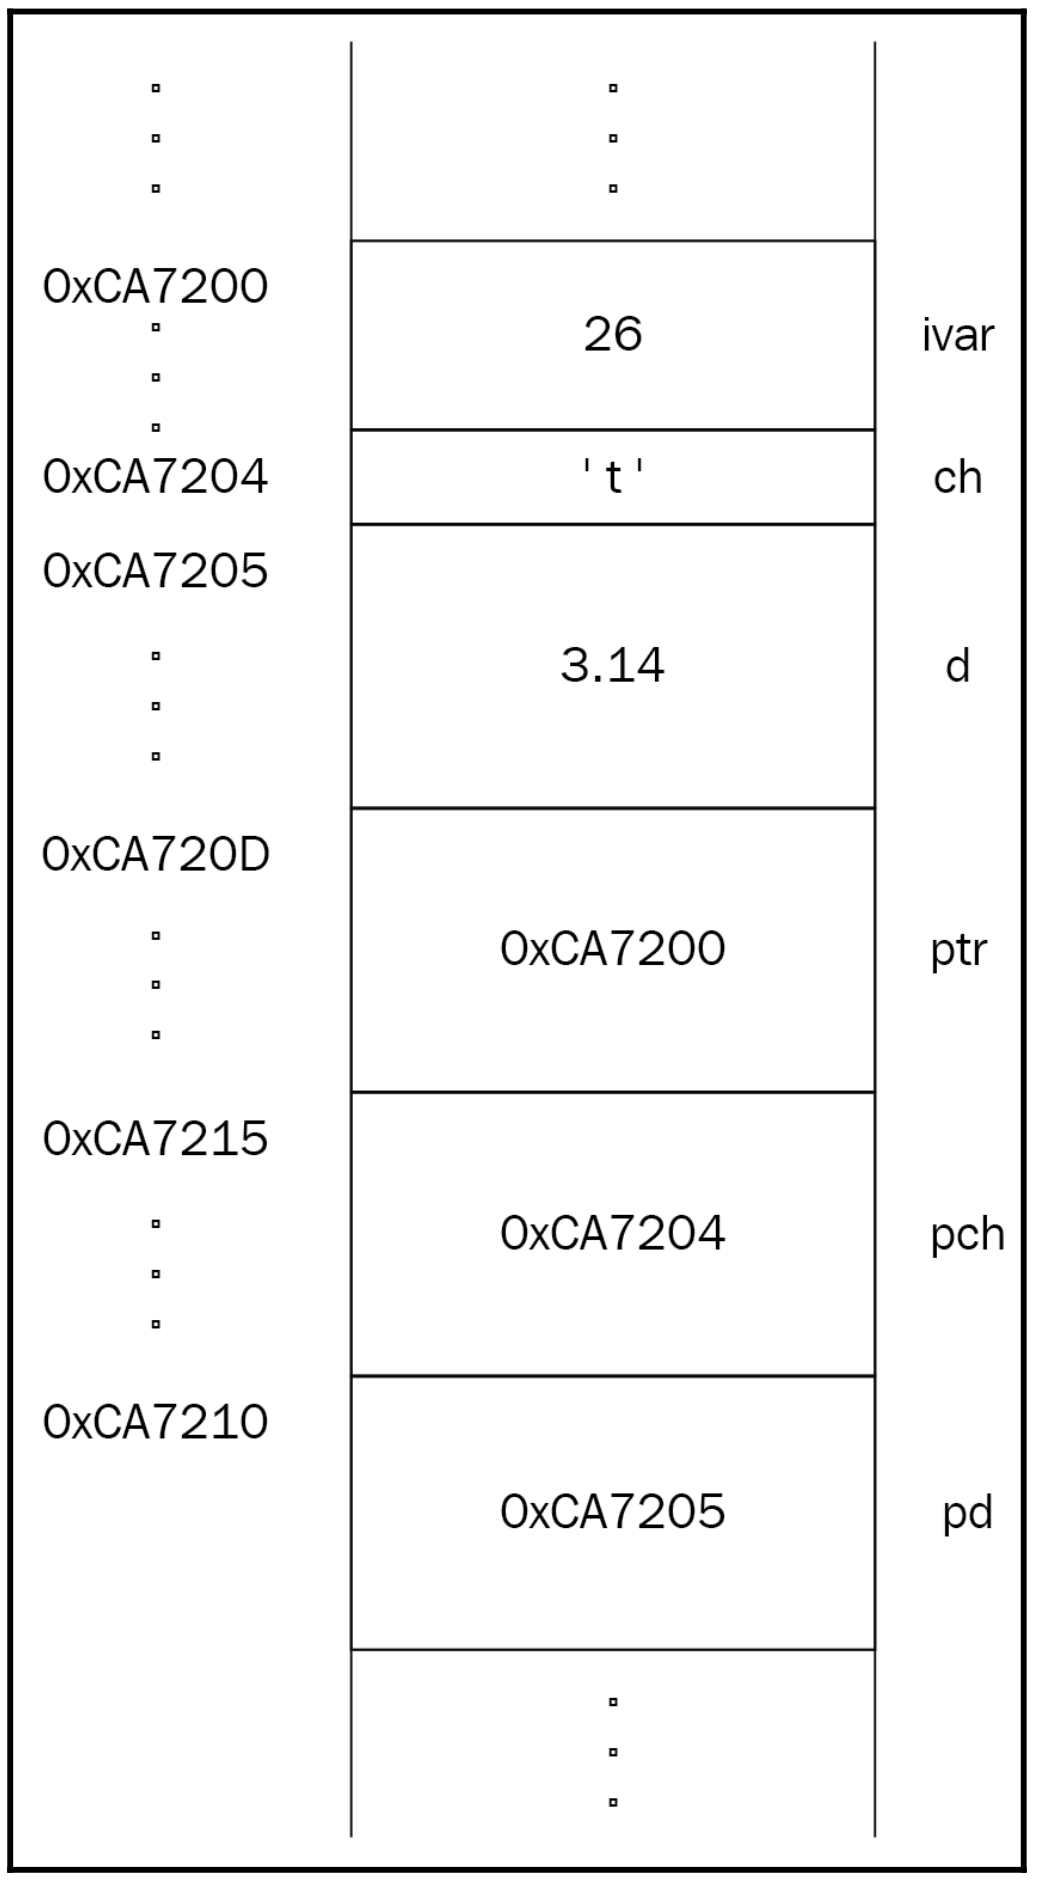
\includegraphics[width=0.5\textwidth]{content/Section-1/Chapter-2/10}
\end{center}

事实证明,在使用指针访问变量时,指针的类型是至关重要。C++提供了解引用操作符(指针名称前的*符号): \par

\begin{lstlisting}[caption={}]
std::cout << *ptr; // prints 26
\end{lstlisting}

它基本上是这样工作的:\par

\begin{enumerate}
	\item 读取指针的内容
	\item 查找与指针中的地址相等的内存单元的地址 
	\item 返回存储在该内存单元中的值
\end{enumerate}

问题是,如果指针指向存储在多个内存单元中的数据,该怎么办?这就是指针类型的作用所在。当对指针进行解引用时,它的类型用于确定应该从它所指向的内存单元读取和返回多少字节。 \par
现在知道了指针存储了变量的第一个字节的地址,实际上可以通过向前移动指针来读取变量的任何字节。我们应该记住地址只是一个数字,所以加上或者减去另一个数字会产生另一个地址。如果我一个char指针指向一个整型变量会怎样? \par

\begin{lstlisting}[caption={}]
int ivar = 26;
char* p = (char*)&ivar;
\end{lstlisting}

当尝试对p指针进行解引用时,它将只返回ivar的第一个字节。\par
现在,如果我们想移动到ivar的下一个字节,我们给char指针加1: \par

\begin{lstlisting}[caption={}]
// the first byte
*p;
// the second byte
*(p + 1);
// the third byte
*(p + 2);
// dangerous stuff, the previous byte
*(p - 1);
\end{lstlisting}

观察下面的图表,它清楚地展示了如何访问ivar:\par

\begin{center}
	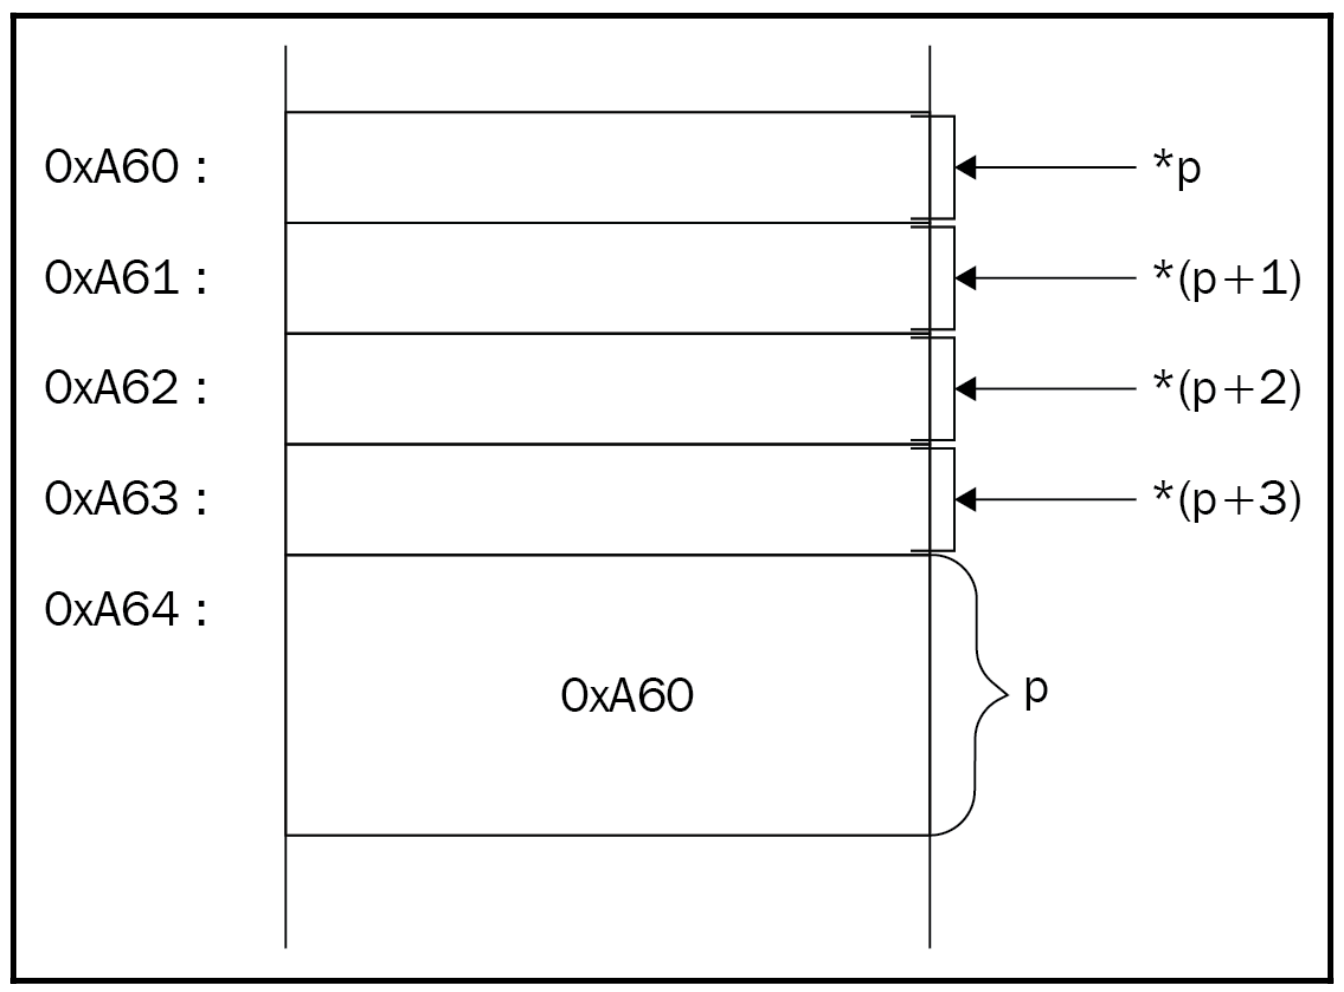
\includegraphics[width=0.5\textwidth]{content/Section-1/Chapter-2/11}
\end{center}

如果你想读取第一个或最后两个字节,你可以使用short类型的指针: \par

\begin{lstlisting}[caption={}]
short* sh = (short*)&ivar;
std::cout << *sh; // print the value in the first two bytes of ivar
std::cout << *(sh + 1); // print the value in the last two bytes of ivar
\end{lstlisting}

\hspace*{\fill} \\ %插入空行

\includegraphics[width=0.05\textwidth]{images/tip}
小心使用指针算术,因为添加或减去一个数字实际上将移动指针,使其与定义的数据类型大小一致。给一个int指针加1将会给实际的地址加上sizeof(int) * 1。 \par
\noindent\textbf{}\ \par

那么指针的大小呢?如前所述,指针只是一个特殊的变量,它可以存储内存地址,并提供返回位于该地址的数据的解引用操作符。因此,如果指针只是一个变量,也应该存储在内存中。我们可以认为char指针的大小小于int指针的大小,因为char类型的长度小于int类型的长度。 \par
关键在于:存储在指针中的数据与指针所指向的数据类型无关。char指针和int指针都存储变量的地址,因此要定义指针的大小,我们应该考虑地址的大小。地址的大小是由系统定义。例如,在32位系统中,地址长度为32位,而在64位系统中,地址长度为64位。这使我们得到一个结论:无论指针指向什么类型的数据,指针的大小都是相同的。\par

\begin{lstlisting}[caption={}]
std::cout << sizeof(ptr) << " = " << sizeof(pch) << " = " << sizeof(pd);
\end{lstlisting}

在32位系统中输出\texttt{4 = 4 = 4},在64位系统中输出\texttt{8 = 8 = 8}。 \par

\noindent\textbf{}\ \par
\textbf{内存段} \ \par
内存由段组成,程序段在加载期间通过这些内存段分布组成,这些人为划分的内存地址范围使操作系统更容易管理程序。二进制文件也可划分为段,如代码和数据,我们前面提到了代码和数据部分。“节”是链接器所需的二进制文件的分割,用于让链接器正常工作,并将用于加载器的节组合成段。 \par
从运行时的角度讨论二进制文件时,我们指的是“段”。数据段包含程序所需和使用的所有数据,而代码段包含处理相同数据的实际指令。当我们提到数据时,并不是指程序中使用的每一个数据。先来看看个例子: \par

\begin{lstlisting}[caption={}]
#include <iostream>
int max(int a, int b) { return a > b ? a : b; }
int main() {
	std::cout << "The maximum of 11 and 22 is: " << max(11, 22);
}
\end{lstlisting}

前面程序的代码段由main()和max()函数的指令组成,其中main()使用cout对象的操作符<<打印消息,然后调用max()函数。哪些数据实际上驻留在数据段中?是否包含max()函数的a和b参数?结果是,数据段中包含的唯一数据是字符串(\texttt{The maximum of 11 and 22 is:}),以及其他静态、全局或常量。我们没有声明任何全局或静态变量,所以唯一的数据就是上述消息。\par
有趣的是11和22的值。这些是文字值,这意味着它们没有地址。因此,它们不在内存中的任何地方。如果它们不在任何地方,那么在程序中位置的唯一就是在代码段中。它们是max()调用指令的一部分。\par
max()函数的a和b参数呢?这里是虚拟内存中的一个段,它负责存储具有自动存储时间的变量——栈。如前所述,堆栈自动处理局部变量和函数参数的内存空间的分配/释放。当max()函数被调用时,参数a和b将位于堆栈中。通常,如果一个对象具有自动存储时间,那么内存空间将在该封闭块的开始处分配。因此,当函数被调用时,参数推入堆栈: \par

\begin{lstlisting}[caption={}]
int max(int a, int b) {
	// allocate space for the "a" argument
	// allocate space for the "b" argument
	return a > b ? a : b;
	// deallocate the space for the "b" argument
	// deallocate the space for the "a" argument
}
\end{lstlisting}

当函数完成时,自动分配的空间将在外围代码块的末尾被释放。 \par

\hspace*{\fill} \\ %插入空行

\includegraphics[width=0.05\textwidth]{images/tip}
外围的代码块不仅表示函数体,还表示条件语句和循环的块。 \par
\noindent\textbf{}\ \par

参数(或局部变量)从堆栈中弹出,“推入”和“弹出”是栈上下文中使用的术语。通过推入堆栈将数据插入到堆栈中,通过弹出堆栈检索(和删除)数据。你可能遇到过“后进先出”这个术语,这完美地描述了栈的推入和弹出操作。\par
当程序运行时,操作系统提供了固定的堆栈大小。栈的大小可以增长,如果它增长到没有剩余空间的程度,程序就会因为栈溢出而崩溃。 \par

\noindent\textbf{}\ \par
\textbf{堆} \ \par
我们将堆栈描述为具有自动存储时间的变量管理器。“自动”这个词意味着程序员不需要关心实际的内存分配和回收。只有在事先知道数据的大小或数据集合的情况下,才能实现自动存储时间。这样编译器就能知道函数参数和局部变量的数量和类型。但是程序倾向于使用动态数据——大小未知的数据。我们将在第5章中详细学习动态内存管理。现在,让我们看看一个简化的内存段图示,看看堆是用来做什么的:\par

\begin{center}
	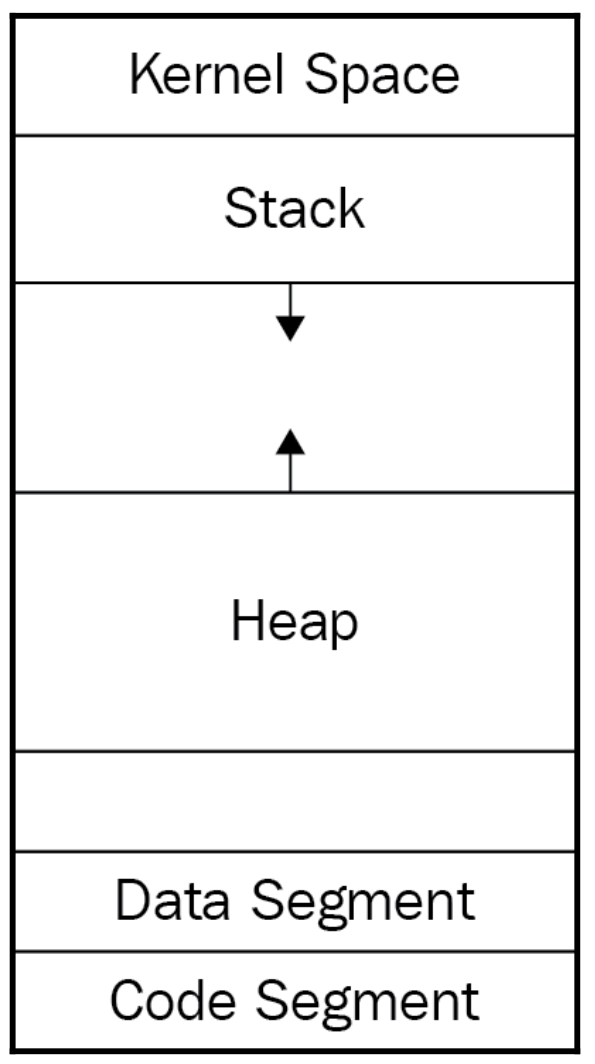
\includegraphics[width=0.3\textwidth]{content/Section-1/Chapter-2/12}
\end{center}

程序使用堆段来请求比以前需要的更多的内存空间,这意味着内存是在程序执行期间动态分配的。无论何时需要,程序都会向操作系统请求新的内存空间。操作系统实际上不知道是整数、用户定义的Point类、甚至是用户定义的Point数组需要内存。程序通过传递所需要字节的实际大小来请求内存。例如,要为Point类型的对象请求一个空间,可以使用malloc()函数: \par

\begin{lstlisting}[caption={}]
#include <cstdlib>
struct Point {
	float x;
	float y;
};
int main() {
	std::malloc(sizeof(Point));
}
\end{lstlisting}

\hspace*{\fill} \\ %插入空行

\includegraphics[width=0.05\textwidth]{images/tip}
malloc()函数来自C语言,为了使用它,需要包含<cstdlib>头文件。\par
\noindent\textbf{}\ \par

malloc()函数分配了一个sizeof(Point)字节的连续内存空间——假设是8个字节。然后,返回该内存的第一个字节的地址,因为这是提供访问空间的唯一方法。问题是,malloc()实际上不知道我们是为Point对象请求内存空间,还是为int对象请求内存空间,它只是返回void*。void*存储已分配内存的第一个字节的地址,但它肯定不能通过对指针的解引用来获取实际数据,因为void没有定义数据的大小。看看下面的图示,它显示了malloc在堆上分配内存:\par

\begin{center}
	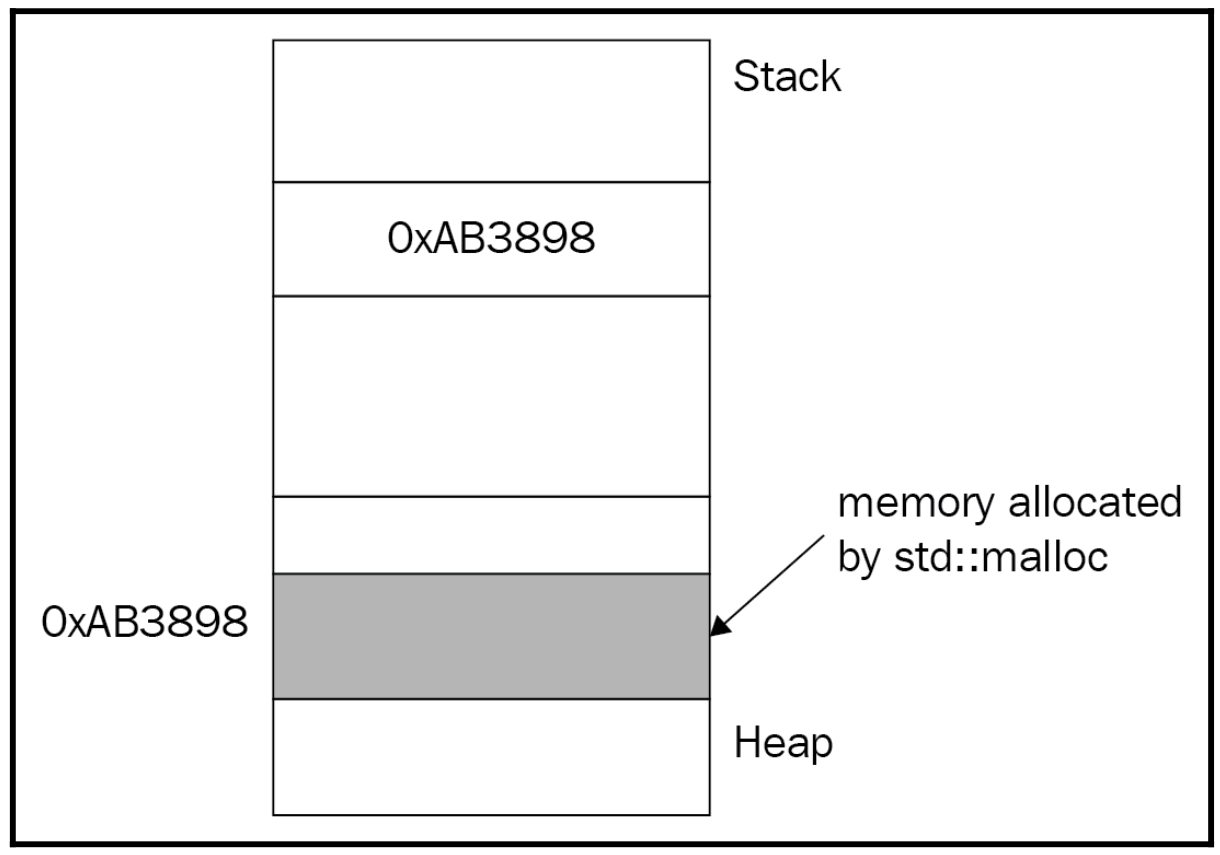
\includegraphics[width=0.5\textwidth]{content/Section-1/Chapter-2/13}
\end{center}

要真正使用内存空间,需要强制转换指向所需类型的void指针:\par

\begin{lstlisting}[caption={}]
void* raw = std::malloc(sizeof(Point));
Point* p = static_cast<Point*>(raw);
\end{lstlisting}

或者,简单地用强制转换结果声明并初始化指针: \par

\begin{lstlisting}[caption={}]
Point* p = static_cast<Point*>(std::malloc(sizeof(Point)));
\end{lstlisting}

C++通过引入new操作符解决了这个难题,该操作符自动获取要分配的内存空间大小,并将结果转换为所需类型:\par

\begin{lstlisting}[caption={}]
Point* p = new Point;
\end{lstlisting}

\hspace*{\fill} \\ %插入空行

\includegraphics[width=0.05\textwidth]{images/tip}
动态内存管理是一个手动过程,如果不再需要内存空间,没有类似于堆栈的结构会自动释放内存空间。要正确管理内存资源,当需要释放内存空间时,应该使用delete操作符。 \par
\noindent\textbf{}\ \par

当访问p指向的Point对象的成员时会发生什么?引用p会返回完整的Point对象,因此要更改成员x的值,应该执行以下操作: \par

\begin{lstlisting}[caption={}]
(*p).x = 0.24;
\end{lstlisting}

或者,更好的是,使用箭头操作符访问: \par

\begin{lstlisting}[caption={}]
p->x = 0.24;
\end{lstlisting}

我们将在第3章中深入研究用户定义类型和结构。\par

\noindent\textbf{}\ \par
\textbf{数组} \ \par
数组是提供连续存储在内存中的数据集合的基本数据结构,许多适配器(如堆栈)都是使用数组实现的。它们的惟一性是数组元素都是同一类型的,这在访问数组元素时起着关键作用。例如,下面的声明创建了一个包含10个整数的数组: \par

\begin{lstlisting}[caption={}]
int arr[]{0, 1, 2, 3, 4, 5, 6, 7, 8, 9};
\end{lstlisting}

数组的名称可退化为指向第一个元素的指针。考虑到数组元素具有相同的类型,我们可以通过将指针指向数组的第一个元素来访问数组的任何元素。例如,下面的代码打印数组的第三个元素: \par

\begin{lstlisting}[caption={}]
std::cout << *(arr + 2);
\end{lstlisting}

第一个元素也是一样,下面三行代码做了同样的事情: \par

\begin{lstlisting}[caption={}]
std::cout << *(arr + 0);
std::cout << *arr;
std::cout << arr[0];
\end{lstlisting}

为了确保arr[2]和*(arr + 2)做同样的事情,我们可以这样做:\par

\begin{lstlisting}[caption={}]
std::cout << *(2 + arr);
\end{lstlisting}

在+后面移动2不会影响结果,所以下面的代码也是有效的:\par

\begin{lstlisting}[caption={}]
std::cout << 2[arr];
\end{lstlisting}

然后输出数组的第三个元素。 \par

访问数组元素的时间复杂度是常量,这意味着访问数组的第一个和最后一个元素的时间是相同的。这是因为每次访问数组元素时,都要执行以下操作: \par

\begin{enumerate}
	\item 通过添加相应的数值来前进指针
	\item 读取放置在指针内存单元的内容 
\end{enumerate}

数组的类型指示应该读(或写)多少内存单元。下面的图表说明了访问时的内存排布: \par

\begin{center}
	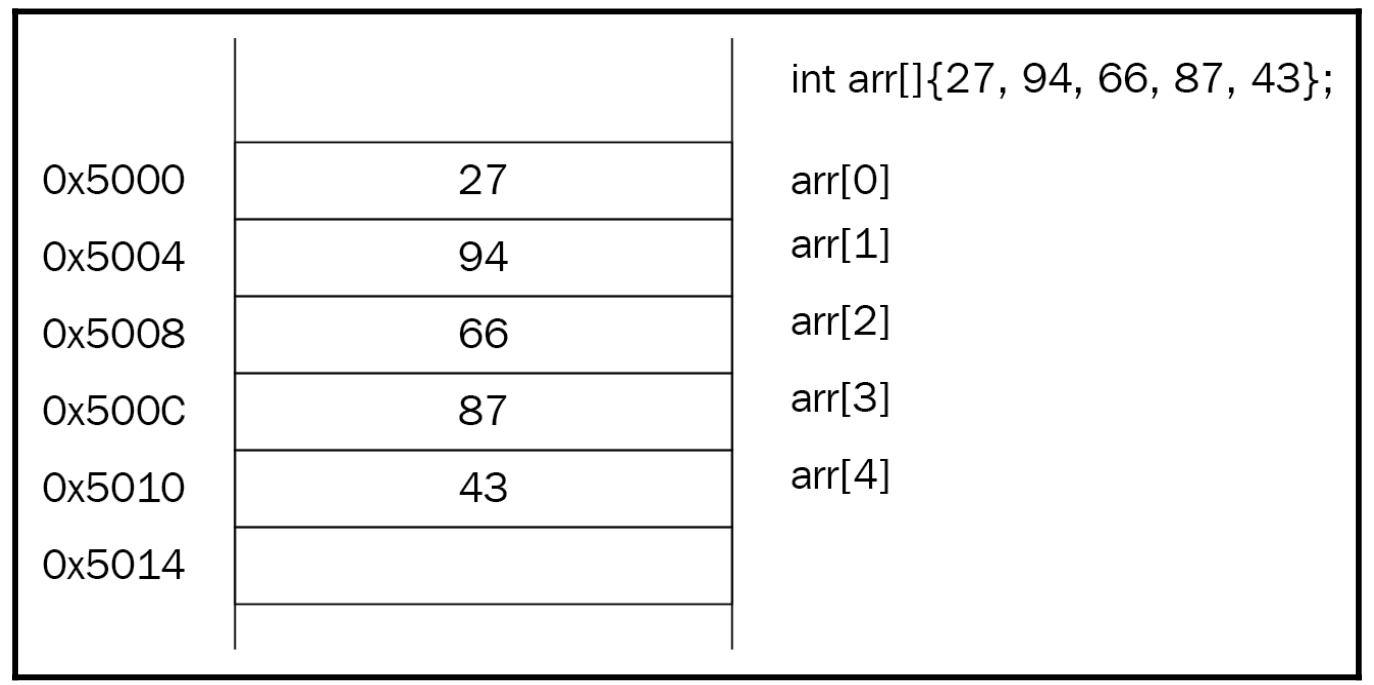
\includegraphics[width=0.5\textwidth]{content/Section-1/Chapter-2/14}
\end{center}

创建动态数组时,这种思想是至关重要的,动态数组是位于堆而不是堆栈中的数组。从堆中分配内存会给出第一个字节的地址,所以访问第一个字节以外的元素的唯一方式是使用指针计算: \par

\begin{lstlisting}[caption={}]
int* arr = new int[10];
arr[4] = 2; // the same as *(arr + 4) = 2
\end{lstlisting}

我们将在第6章进一步讨论数组和其他数据结构。 \par

\noindent\textbf{}\ \par
\textbf{控制流} \ \par
所有编程语言的最基本概念都是条件语句和循环。\par

\noindent\textbf{}\ \par
\textbf{条件} \ \par
很难想象一个程序不包含条件语句。检查函数的输入参数以确保它们的安全执行几乎是一种习惯。例如,divide()函数接受两个参数,将其中一个除以另一个,并返回结果。很明显,我们需要确保除数不为零: \par

\begin{lstlisting}[caption={}]
int divide(int a, int b) {
	if (b == 0) {
		throw std::invalid_argument("The divisor is zero");
	}
	return a / b;
}
\end{lstlisting}

条件语句是编程语言的核心。毕竟,一个程序是行动和决定的集合。例如,下面的代码使用条件语句来查找两个输入参数中的最大值: \par

\begin{lstlisting}[caption={}]
int max(int a, int b) {
	int max;
	if (a > b) {
		// the if block
		max = a;
	} else {
		// the else block
		max = b;
	}
	return max;
}
\end{lstlisting}

为了表达if-else语句的用法,上面的例子过分简化了。然而,我们最感兴趣的是这样一个条件语句的实现。当遇到if语句时,编译器会生成什么?CPU依次执行指令,指令是只做一件事的简单命令。高级编程语言(如C++)中,我们可以在一行中使用复杂的表达式,而汇编指令是简单的命令,在一个循环中只能执行一个简单的操作:移动、添加、减去等。 \par
CPU从代码内存段获取指令,解码找出应该做什么(移动数据,加数字,减数字),然后执行命令。 \par
为了以最快的速度运行,CPU将操作数和执行结果存储在称为寄存器的存储单元中。你可以把寄存器看作是CPU的临时变量,寄存器是位于CPU内的物理内存单元,因此比访问RAM快得多。为了从汇编语言程序中访问寄存器,我们使用它们的指定名称,如:rax、rbx、rdx等。CPU命令操作寄存器而不是RAM单元,这就是为什么CPU必须将变量的内容从内存复制到寄存器,执行操作并将结果存储在寄存器中,然后将寄存器的值复制回内存单元。 \par
例如,下面的C++表达式只需要一行代码: \par

\begin{lstlisting}[caption={}]
a = b + 2 * c - 1;
\end{lstlisting}

汇编表示如下(在分号之后添加注释): \par

\begin{lstlisting}[caption={}]
mov rax, b; copy the contents of "b"
          ; located in the memory to the register rax
mov rbx, c; the same for the "c" to be able to calculate 2 * c
mul rbx, 2; multiply the value of the rbx register with
          ; immediate value 2 (2 * c)
add rax, rbx; add rax (b) with rbx (2*c) and store back in the rax
sub rax, 1; subtract 1 from rax
mov a, rax; copy the contents of rax to the "a" located in the memory
\end{lstlisting}

条件语句会跳过部分代码。例如,调用max(11,22)意味着if块将被省略。为了在汇编语言中表达这一点,使用了跳转的思想。我们比较两个值,并根据结果跳转到代码的指定部分。我们对这部分进行标记,以使找到指令集成为可能。例如,要跳过向寄存器rbx添加42,我们可以使用无条件跳转指令jp跳转到标记为UNANSWERED的部分,如下所示: \par

\begin{lstlisting}[caption={}]
mov rax, 2
mov rbx, 0
jmp UNANSWERED
add rbx, 42; will be skipped
UNANSWERED:
add rax, 1
; ...
\end{lstlisting}

jmp指令执行无条件跳转,指定的标号处开始执行第一条指令,而不进行任何条件检查。CPU也提供了条件跳转,max()函数的函数体将转换为以下的汇编代码(简化),其中jg和jle命令分别被解释为大于时跳转,小于或等于时跳转(基于使用cmp指令进行比较的结果):\par

\begin{lstlisting}[caption={}]
mov rax, max; copy the "max" into the rax register
mov rbx, a
mov rdx, b
cmp rbx, rdx; compare the values of rbx and rdx (a and b)
jg GREATER; jump if rbx is greater than rdx (a > b)
jl LESSOREQUAL; jump if rbx is lesser than
GREATER:
mov rax, rbx; max = a
LESSOREQUAL:
mov rax, rdx; max = b
\end{lstlisting}

前面的代码中,标签GREATER和LESSOREQUAL表示前面实现的max()函数的if和else子句。 \par

\noindent\textbf{}\ \par
\textbf{switch语句} \ \par
switch语句等条件语句使用的逻辑如下所示: \par

\begin{lstlisting}[caption={}]
switch (age) {
	case 18:
		can_drink = false;
		can_code = true;
		break;
	case 21:
		can_drink = true;
		can_code = true;
		break;
	default:
		can_drink = false;
}
\end{lstlisting}

假设rax代表年龄,rbx代表can\underline{ }drink, rdx代表can\underline{ }code。前面的例子将转化为下面的汇编指令(简化以表达基本思想): \par

\begin{lstlisting}[caption={}]
cmp rax, 18
je CASE_18
cmp rax, 21
je CASE_21
je CASE_DEFAULT
CASE_18:
	mov rbx, 0; cannot drink
	mov rdx, 1; can code
	jmp BEYOND_SWITCH; break
CASE_21:
	mov rbx, 1
	mov rdx, 1
	jmp BEYOND_SWITCH
CASE_DEFAULT:
	mov rbx, 0
BEYOND_SWITCH:
	; ....
\end{lstlisting}

每个break语句都转换为跳转到BEYOND\underline{ }SWITCH标签,因此,如果我们忘记break关键字,例如:在age为18的情况下,执行也会跳转到case\underline{ }21。 \par

让我们找种方法来避免在源代码中使用条件语句,这样既可以使代码更短,也可能更快——函数指针。 \par

\noindent\textbf{}\ \par
\textbf{用函数指针替换条件语句} \ \par
前面,我们研究了内存段,其中最重要的是代码段(也称为文本段)。这个段包含程序映像,它是应该执行的程序的指令。指令通常分组成函数,函数提供了名称,允许我们从其他函数中调用它们。函数存储在可执行文件的代码段中。\par
函数有它自己的地址。可以声明一个接受函数地址的指针,然后在后面调用该函数: \par

\begin{lstlisting}[caption={}]
int get_answer() { return 42; }
int (*fp)() = &get_answer;
// int (*fp)() = get_answer; same as &get_answer
\end{lstlisting}

函数指针的调用方式与普通函数相同: \par

\begin{lstlisting}[caption={}]
get_answer(); // returns 42
fp(); // returns 42
\end{lstlisting}

假设我们正在编写一个程序,从输入中获取两个数字和一个字符,并对这些数字执行算术运算。操作由字符指定,可以是+、-、*或/。我们实现了四个函数:add()、subtract()、multiply()和divide(),并根据输入的字符的值调用其中一个函数。 \par
我们不需要在一堆if语句或switch语句中检查字符的值,而是使用哈希表将操作类型映射到指定的函数: \par

\begin{lstlisting}[caption={}]
#include <unordered_map>
int add(int a, int b) { return a + b; }
int subtract(int a, int b) { return a - b; }
int multiply(int a, int b) { return a * b; }
int divide(int a, int b) { return (b == 0) ? 0 : a / b; }
int main() {
	std::unordered_map<char, int (*)(int, int)> operations;
	operations['+'] = &add;
	operations['-'] = &subtract;
	operations['*'] = &multiply;
	operations['/'] = &divide;
	// read the input
	char op;
	int num1, num2;
	std::cin >> num1 >> num2 >> op;
	// perform the operation, as follows
	operations[op](num1, num2);
}
\end{lstlisting}

std::unordered\underline{ }map将char映射到定义为(*)(int, int)的函数指针。也就是说,可以指向任何接受两个整数并返回一个整数的函数。 \par

\hspace*{\fill} \\ %插入空行

\includegraphics[width=0.05\textwidth]{images/tip}
哈希表由std::unordered\underline{ }map表示,定义在<unordered\_map>头文件中。\par
\noindent\textbf{}\ \par

现在我们不需要这样写: \par

\begin{lstlisting}[caption={}]
if (op == '+') {
	add(num1, num2);
} else if (op == '-') {
	subtract(num1, num2);
} else if (op == '*') {
	...
\end{lstlisting}

我们只需调用由字符映射的函数: \par

\begin{lstlisting}[caption={}]
operations[op](num1, num2);
\end{lstlisting}

\hspace*{\fill} \\ %插入空行

\includegraphics[width=0.05\textwidth]{images/tip}
尽管哈希表的使用很漂亮,看起来也更专业,但应该注意一些意想不到的情况,比如:无效的输入。 \par
\noindent\textbf{}\ \par

\noindent\textbf{}\ \par
\textbf{函数类型} \ \par
unordered\underline{ }map的第二个参数是int (*)(int, int),字面意思是指向函数的指针,该函数接受两个整数并返回一个整数。C++支持类模板std::function作为通用函数包装器,允许存储可调用对象,包括普通函数、lambda表达式、函数对象等。存储的对象称为std::function的目标,如果没有目标,将在调用时抛出std::bad\underline{ }function\underline{ }call异常。这有助于使哈希表接受任何可调用对象作为第二个参数,并处理异常情况,如前面提到的无效字符输入。 \par
下面的代码段说明了这一点: \par

\begin{lstlisting}[caption={}]
#include <functional>
#include <unordered_map>
// add, subtract, multiply and divide declarations omitted for brevity
int main() {
	std::unordered_map<char, std::function<int(int, int)> > operations;
	operations['+'] = &add;
	// ...
}
\end{lstlisting}

注意std::function的参数,它的形式是int(int, int),而不是int(*)(int, int)。使用std::function可以帮助我们处理异常情况。例如,\texttt{operations['x'](num1, num2);}将导致创建一个映射到字符x的空std::function。 \par
并且调用它会抛出异常,所以可以通过正确处理调用来确保代码的安全性: \par

\begin{lstlisting}[caption={}]
// code omitted for brevity
std::cin >> num1 >> num2 >> op;
try {
	operations[op](num1, num2);
} catch (std::bad_function_call e) {
	// handle the exception
	std::cout << "Invalid operation";
}
\end{lstlisting}

最后,我们可以使用lambda表达式——在适当位置构造的未命名函数,并能够捕获作用域中的变量。例如,可以将lambda表达式插入到哈希表之前创建一个lambda表达式,而不是声明上述函数,然后将它们插入到哈希表中: \par

\begin{lstlisting}[caption={}]
std::unordered_map<char, std::function<int(int, int)> > operations;
operations['+'] = [](int a, int b) { return a + b; }
operations['-'] = [](int a, int b) { return a * b; }
// ...
std::cin >> num1 >> num2 >> op;
try {
	operations[op](num1, num2);
} catch (std::bad_functional_call e) {
	// ...
}
\end{lstlisting}

lambda表达式将贯穿全书。

\noindent\textbf{}\ \par
\textbf{循环} \ \par
循环可以认为是可重复的if语句,同样应该转换成CPU比较和跳转指令。例如,我们可以使用while循环计算从0到10的数字总和: \par

\begin{lstlisting}[caption={}]
auto num = 0;
auto sum = 0;
while (num <= 10) {
	sum += num;
	++num;
}
\end{lstlisting}

这将转译成以下的汇编代码(简化): \par

\begin{lstlisting}[caption={}]
mov rax, 0; the sum
mov rcx, 0; the num
LOOP:
	cmp rbx, 10
	jg END; jump to the END if num is greater than 10
	add rax, rcx; add to sum
	inc rcx; increment num
	jmp LOOP; repeat
END:
	...
\end{lstlisting}

C++17引入了init语句,可以在条件语句和循环中使用。在while循环外声明的num变量现在可以移动到循环中: \par

\begin{lstlisting}[caption={}]
auto sum = 0;
while (auto num = 0; num <= 10) {
	sum += num;
	++num;
}
\end{lstlisting}

同样的规则也适用于if语句,例如: \par

\begin{lstlisting}[caption={}]
int get_absolute(int num) {
	if (int neg = -num; neg < 0) {
		return -neg;
	}
	return num;
}
\end{lstlisting}

C++ 11引入了基于范围的for循环,使得语法更加清晰。例如,让我们使用新的for循环调用前面定义的所有算术运算: \par

\begin{lstlisting}[caption={}]
for (auto& op: operations) {
	std::cout << op.second(num1, num2);
}
\end{lstlisting}

迭代unordered\underline{ }map返回一个pair,其中包含二个成员,第一个是键,第二个是映射到该键的值。C++ 17更进一步,允许我们编写如下相同的循环: \par

\begin{lstlisting}[caption={}]
for (auto& [op, func]: operations) {
	std::cout << func(num1, num2);
}
\end{lstlisting}

了解编译器实际生成的过程,是设计和实现高效软件的关键。我们讨论了条件语句和循环的底层细节,它们几乎是每个程序的基础。 \par

\noindent\textbf{}\ \par
\textbf{总结} \ \par
这一章中,我们介绍了程序执行的细节。我们讨论了函数和main()函数的一些特性。我们了解了递归是如何工作的,以及main()函数不能递归调用。 \par
由于C++支持底层编程概念(如通过地址访问内存字节)的少数高级语言之一,我们研究了数据如何驻留在内存中,以及如何在访问数据时结合指针。对于专业C++程序员来说,了解这些细节是必须的。 \par
最后,我们从汇编语言的角度讨论了条件语句和循环的主题。在这一章中,我们介绍了C++20的特性。 \par
下一章中,我们将学习更多关于面向对象编程(OOP)的知识,包括语言对象模型的内部细节。我们将深入虚函数的细节,并了解如何使用多态性。 \par

\noindent\textbf{}\ \par
\textbf{问题} \ \par
\begin{enumerate}
	\item main()函数有多少个形参?
	\item constexpr说明符用于什么?
	\item 为什么建议使用迭代而不是递归?
	\item 栈和堆的区别是什么?
	\item 如果ptr声明为int*,它的大小是多少? 
	\item 为什么将访问数组元素视为常量时间操作?
	\item switch语句中,如果忘记break会发生什么?
	\item 如何将算术操作示例中的multiply()和divide()函数实现为lambda表达式?
\end{enumerate}

\noindent\textbf{}\ \par
\textbf{扩展阅读} \ \par
你可以参考下面的书获得更多关于本章主题的信息: 《C++ High Performance》,Viktor Sehr和Bjorn Andrist ( https:/​/​www.​amazon.
com/​gp/​product/​1787120953 ).\par

\newpage